%!TEX program = pdflatex
\documentclass[submission,copyright]{eptcs}
\providecommand{\event}{QAPL 2016} % Name of the event you are submitting to
\usepackage{breakurl}             % Not needed if you use pdflatex only.

\usepackage{amsmath}
\usepackage{amssymb}
\usepackage[nolist]{acronym}
\usepackage[english]{babel}
\usepackage[lined,boxed,linesnumbered,ruled]{algorithm2e}
\usepackage{mathrsfs}
\usepackage{graphicx}
\usepackage{url}
\usepackage{wrapfig}
\usepackage{thmtools,thm-restate,amsthm}


\usepackage{tikz} % DISEGNI
\usetikzlibrary{shapes}
\usetikzlibrary{arrows}
\usetikzlibrary{backgrounds}
\usetikzlibrary{positioning}

\DeclareMathOperator*{\argmax}{arg\,max} % \argmax_
\DeclareMathOperator*{\argmin}{arg\,min} % \argmin_

% === ACRONYMS LIST ===
\begin{acronym}
  \acro{LTS}{Labeled Transition System}
  \acro{DTMC}{Discrete-Time Markov Chain}
  \acro{MDP}{Markov Decision Process}
  \acro{BMDP}{Belief Markov Decision Process}
  \acro{HMM}{Hidden Markov Model}
  \acro{BMC}{Belief Markov Chain}
  \acro{POMDP}{Partially Observable Markov Decision Process}
  \acro{LTL}{Linear Temporal Logic}
  \acro{DRA}{Deterministic Rabin Automaton}
  \acro{NBA}{Nondeterministic B\"uchi Automaton}
\end{acronym}

\acrodefplural{LTS}[LTSs]{Labeled Transition Systems}
\acrodefplural{DTMC}[DTMCs]{Discrete-Time Markov Chains}
\acrodefplural{MDP}[MDPs]{Markov Decision Processes}
\acrodefplural{BMDP}[BMDPs]{Belief Markov Decision Processes}
\acrodefplural{HMM}[HMMs]{Hidden Markov Models}
\acrodefplural{BMC}[BMCs]{Belief Markov Chains}
\acrodefplural{POMDP}[POMDPs]{Partially Observable Markov Decision Processes}
\acrodefplural{DRA}{Deterministic Rabin Automata}
\acrodefplural{NBA}{Nondeterministic B\"uchi Automata}

% Theorem Styles
\newtheorem{theorem}{Theorem}
\newtheorem{lemma}[theorem]{Lemma}
\newtheorem{proposition}[theorem]{Proposition}
\newtheorem{corollary}[theorem]{Corollary}
% Definition Styles
\theoremstyle{definition}
\newtheorem{definition}[theorem]{Definition}
\newtheorem{example}{Example}
\theoremstyle{remark}
\newtheorem{remark}{Remark}

\title{Adaptation in partially observable environments via model checking}
\author{Rocco De Nicola
\institute{IMT Institute for Advanced Studies Lucca, Italy}
\email{\quad rocco.denicola@imtlucca.it}
\and
Michele Loreti 
\institute{Universit\`a degli Studi di Firenze, Italy}
\email{michele.loreti@unifi.it}
\and
Marco Tinacci
\institute{IMT Institute for Advanced Studies Lucca, Italy}
\email{marco.tinacci@imtlucca.it}
}
\def\titlerunning{Adaptation in partially observable environments via model checking}
\def\authorrunning{R. De Nicola, M. Loreti \& M. Tinacci}

\begin{document}
\maketitle

% === SECTIONS ===
%!TEX root = main.tex

\begin{abstract}
Modern software systems consist of a large number of agents that cooperate and compete
to achieve \emph{local} and \emph{global} goals. Local goals are specific of single agents
while the global ones refer to the expected emerging behaviour resulting from the interaction of many agents. 
Agents are often located in an environment that can impact on their \emph{goals}.  
For this reason it is crucial to have mechanisms that allow each agent to adapt its behaviour to
the changing environmental conditions while guaranteeing goals achievement. When a change in the environment is perceived, each agent has to use its knowledge to perform specific actions and \emph{adapt} its behaviour.
Unfortunately, only in rare cases agents have a complete view of the context where they are operating;  often only a partial view is available. 
In this paper we show how formal tools, and specifically probabilistic model checking, can be used 
to support dynamic adaptation of agents when only a partial \emph{observations} of the environment are available. 
The proposed approach guarantees that each agent is  able to select those \emph{adaptation actions} that
maximizes the probability of achieving the required goal.
In the paper, system behaviour is described in terms of POMDP (Partial Observable Markov Decision Processes)
while goals are specified using an appropriate variant of LTL.  
A simple running example, based on a simple robotic scenario, is used to show the effectiveness of the proposed approach.
\end{abstract}




%!TEX root = main.tex

\section{Introduction} % (fold)
\label{sec:introduction}

Many modern software systems consist of a large number of agents that cooperate and compete \cite{}
to achieve \emph{local} and \emph{global} goals. Local goals are specific of single agents
while the global ones refer to the expected emerging behaviour resulting from the interaction of many agents. 
Agents are often located in an environment that can impact on their \emph{goals}.  
For this reason it is crucial to have mechanisms that allow each agent to adapt its behaviour to
the changing environmental conditions while guaranteeing goals achievement. When a change in the environment is perceived, each agent has to use its knowledge to perform specific actions and \emph{adapt} its behaviour.
Unfortunately, only in rare cases agents have a complete view of the context where they are operating;  often only a partial view is available.  It is then important to develop tools to be used 
to support dynamic adaptation of agents also in presence of partial information about the operating environment.

\paragraph{Adaptive systems} % (fold)
\label{par:adaptive_systems}
The issue of programming adaptive agents is present in many scenarios. Typically, each adaptive agent 
%knows its own features but it 
does not have complete information of the activities taking place in the surrounding environment. 
Thus, 
%Since it has a partial knowledge of the environment, 
methodologies are needed to take decisions to adapt to circumstances. The information about the state of the environment are usually stored in a set of \emph{control data} that are used for \emph{adaptation}. A system is said to be adaptive when its behaviour and its run-time decisions depend directly upon this set of \emph{control data}~\cite{BruniCGLV12}.

Examples of adaptive systems involve agents like robots that have to navigate towards a light source, gather resources, rescue victims while avoiding to fall into traps or to interfere with each other.
% Examples of adaptive systems are swarms of robots, coordinating to reach specific goal like navigating towards a light source, gathering resources, rescuing victims, \ldots \  while avoiding traps or collisions between components of the swarm.
Another example  can be found in cloud computing scenarios where physical machines have to adapt in order to guarantee availability of specific virtual ones while guaranteeing availability and quality of service parameters agreed with the clients. 
% A third example of adaptive systems are electrical car fleets that by exploiting exchange of messages whenever possible have to optimize at run time the transport of people, the use of parking lots or of charging stations while taking into account traffic situation and timing constraints.
%
% agent/environment approach
%In these scenarios, components interact with the other entities in the environment in which they are operating but have only a limited knowledge of the environment itself and of the status of other components.
% paragraph adaptive_systems (end)

\paragraph{Methodology} % (fold)
\label{par:methodology}
% general approach
In this paper, we propose a general methodology to be used when dealing with adaptive agents that interacts with an external environment by executing actions and perceiving signals. The environment is formed by all the components that are external to the agent; the controller of each agent exploits the observable history (sequences of actions and observations) to decide the action to perform in order to achieve the specific target in an optimal way. The target is formally specified at design-time by means of a temporal logic formula  that expresses properties of observation sequences in probabilistic and partially observable domains. A methodology is introduced to resolve agents' choices by relying on model checking~\cite{Katoen-Baier};  the action to be performed are determined by taking into account the path that maximizes the probability of satisfying the provided target formula.

We consider systems whose behaviour is fully described but such that their current state is 
%not directly (partially) 
only partially observable. Agents are described by means of  nondeterministic models and the environment with probabilistic ones. By composing these two systems we obtain a partially observable process in which every state is split in two parts: the controller, that is fully observable, and the environment, that is not directly observable. The history of performed actions and perceived observations is used to refine a probabilistic belief about the current state.

The classical model checking algorithm is ``adapted'' to partially observable models in order to check the probabilities to satisfy the temporal logic formula that describes the goal. The partially observable model is transformed into a fully observable one, observations are used to label states and the measure of satisfiability of a property is reduced to the one in a fully observable context. The adaptation strategy consists then in choosing the action that maximize the chances to satisfy the goal formula. Depending on the needs, it might be appropriate to minimize the risk or to maximize the opportunities. %Synthesizing these kind of strategies intrinsically ensure a correct behaviour with respect to the chosen goal formula.

% runtime
Since the (storage and computing)  resources available to the agents are often limited, the model checking approach may look expensive. But, it has to be considered that, we rely on a two steps  algorithm; the first step has an exponential complexity while the second one is polynomial.  The former one is computed just once and only the latter
%, that is the interaction with the environment, 
has to be computed at run-time. 

% paragraph methodology (end)

\paragraph{A running example} % (fold)
\label{par:a_running_example}

\setlength\intextsep{0pt}
\begin{wrapfigure}[15]{r}{0.3\textwidth}	
%\vspace{-1cm}
%\begin{figure}[htb]
	\begin{center}
	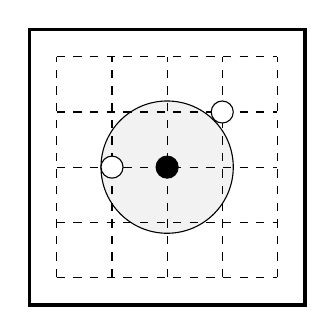
\begin{tikzpicture}[scale=.7]
	\begin{scope}
%	  \filldraw [fill=gray!10] (4,4) circle (1.4); % raggio esteso
	  \filldraw [fill=gray!10] (3,3) circle (1.2); % raggio ridotto
	
	  \draw[dashed] (1, 1) grid (5, 5);
	  \draw[very thick, scale=1] (0.5, 0.5) rectangle (5.5, 5.5);
	
	  \filldraw [fill=black!100] (3,3) circle (0.2);
		
	  \filldraw [fill=white!50] (4,4) circle (0.2);
	  \filldraw [fill=white!50] (2,3) circle (0.2);
%	  \filldraw [fill=white!50] (2,2) circle (0.2);
	\end{scope}
	\end{tikzpicture}
	\end{center}
	\caption{Bird's-eye view representation of the robot arena scenario}
	\label{fig:arenarobot}
%\end{figure}
%\vspace{-.71cm}
\end{wrapfigure}

In the paper we will use a simple robotic scenario as a running example. We consider a robot that moves inside an arena with other robots. %has to reach a destination avoiding other robots or obstacles. 
The proximity sensors of the robot analyse the surrounding area to locate obstacles and their positions; the acquired information is then used by the robot to determine the direction to take.

Figure~\ref{fig:arenarobot} provides a pictorial rendering of the scenario; the arena is represented as a $5\times 5$ grid and is bounded by four walls. The dashed grid represents the agents' walkable paths. %the paths walkable by agents.
We assume that at any step a robot can move from a cross to an adjacent one.
The arena contains four agents; the main robot, the black one, and three white robots that, it is assumed, follow a random trajectory. The main robot monitors the five local positions (north, south, east, west and the central position) via proximity sensors. It is able to perceive other agents within a range of visibility represented by a gray circle; in the figure, it can perceive just one agent at west.

In this kind of setting we may want to attribute different goals to the black robot, like collision-avoidance or tracking the white robots' movement. We use this simple scenario to show how goals can be formally represented and, starting from them, how good the results obtained by the synthesis of an adaptive controller are.
%are the results obtained by the synthesis of an adaptive controller.

% example application
%Let's consider the case in which the robot has to reach a given target position minimizing the number of collisions with other robots or obstacles, we can imagine a system composed by the main agent (the robot) running in parallel with the environment. The environment will be composed by the other robots and by the obstacles that the adaptive robot is able to recognize. When the choice to be taken is related to the direction to follow, the model checker will be used to calculate the probabilities, for each possible local decision, of not colliding with other robots within a certain number of steps. In this way the success probability for each available choice can be determined and then the robot knows that the action to be executed is the one with the highest associated probability.

% paragraph a_running_example (end)

%\paragraph{Literature review} % (fold)
%\label{par:literature_review}
%
%% adaptive systems formalization
%%This work focuses on a formal technique to model several features of an adaptive system. To do that we take inspiration from \cite{Bruni2013} and we model agents' behaviours with transition systems composed together into the global system's behaviour. The most important distinction we make is the one between the adaptive agent and the surrounding environment: the former can be controlled by external actions while the latter may be the result of a further composition among many behaviours of other components.
%%
%%% CSP
%%Communication between adaptive agent and environment works as synchronisation between processes in CSP \cite{BrookesHR84,DengGHM08}, indeed all the components of the system are modeled as parallel processes communicating with each other.
%%The agent's behaviour consists in sending messages to the environment that is always ready to accept incoming requests. This assumption makes the action execution non-blocking for the agent. Moreover, the environment may react in different ways depending on the received message. We have then a two side communication between the adaptive agent and the environment, that is in turn the result of the parallel composition of the behaviour of every external component.
%%\\
%
%% partially observable models
%Partially observable models like \acp{HMM} \cite{Rabiner90} and \acp{POMDP}~\cite{cassandra1998survey} have been successfully employed in many fields like speech-recognition~\cite{Rabiner90} and activity recognition for ambient assisted living~\cite{vicario2015continuous}.
%These models cope with the lack of information typical of an adaptive system. In particular \acp{POMDP} give the possibility to model the partial knowledge in presence of input and output interactions, as sensing and acting procedures. Finding the optimal scheduler is a problem that has been approached in different ways~\cite{LittmanCK95} since many theoretical limits have been proven to subsist: building the optimal scheduler function is PSPACE-complete in case of finite horizon~\cite{Papadimitriou1987} and determining its existence is undecidable for infinite horizon~\cite{MadaniHC99}.
%
%% model checking on partially observable models
%Model checking on \acp{HMM} is proposed in~\cite{ZhangHJ05} together with the extended definitions of branching-time and linear-time logics to include belief states and observation specifications. In this work we adopt a different perspective and we consider observations as label of states. We use classic \ac{LTL} formulae~\cite{Pnueli77} to express properties with probabilistic observations on \acp{POMDP}. 
%
%We want to employ model checking techniques to solve a planning problem, this kind of approach has already been proposed in a similar way in~\cite{Bertoli2001,LagoPT02}. In~\cite{Bertoli2001} the model checking techniques are employed to solve a planning problem, we further exploit the classical algorithm to solve the same problem at run-time. Also the logic used to formulate agent's objectives differs from the goal language proposed in~\cite{LagoPT02} since we focus on the explicit use of observation signals.
%
%%Linear-time model checking on \acp{POMDP} is just one step toward our aim, that is building a scheduler given an \ac{LTL} formula that describe the objective of the adaptive agent. Indeed, given a formula and the formal model of the system we can reuse the \ac{LTL} model checking algorithm to automatize the computation of a scheduler that can control the adaptive agent.
%
%% paragraph literature_review (end)

\paragraph{Structure of the paper} % (fold)
\label{par:structure_of_the_paper}
The rest of the paper is organized as follows. We start by introducing the basic structures and languages that we have chosen
%with preliminaries models, \acp{DTMC}, \acp{MDP} and \acp{POMDP} that are the chosen structures 
to represent agents' behaviour and environment; then we extend them to model the adaptation problem and  
%comprehensive of a \ac{LTL} 
to express goals. Subsequently, we prove correctness of the proposed transformations, present the adaptation algorithm, split into an off-line and on-line phase, and discuss its complexity. Finally, we show some results of the proposed method applied to the robotics example.
% and to a cloud computing scenario.

% paragraph structure_of_the_paper (end)

% section introduction (end)

%!TEX root = main.tex

\section{Background} % (fold)
\label{sec:preliminaries}

In this section we introduce the preliminary concepts that provide the foundational base for the proposed approach. First we will recall basic definitions of \ac{LTS}, \ac{DTMC} and \acp{MDP}. Then we consider the partially observable extensions of the last two models that are, respectively, \acp{HMM} and \acp{POMDP}.

In this paper we will use the following notation: $[i..j] \equiv i,i+1,\dots,j-1,j$ represents the sequence of natural numbers from $i$ to $j$, $[..j] \equiv [0..j]$, $\Delta(X)$ is the set of all the discrete probability distributions over any domain $X$ and $Y^\omega$ is the set of all the infinite sequences of elements of $Y$. We will adopt a name-space structure to ease the notation, when a structure defined as $X = \langle Y \rangle$ we can univocally index the internal element as $Y_X$. We omit the index when it is clear from the context.

Since we need to describe different kinds of paths for different models, we introduce a uniform notation. Let $Paths^X$ be the set of infinite paths of a model $X$, we denote with $FPaths^X$ the set of prefixes of every path in $Paths^X$. Let $\pi = \pi_0, \pi_1, \dots$ be a path in $Paths^X$ where every element $\pi_i = (y_0,y_1,\dots,y_n) \in Y_0 \times Y_1 \times \dots \times Y_n$ ($i = 0,1,\dots$) is a tuple of elements $y_i$ from sets $Y_j$ ($j=0,1,\dots,n$), we denote with $\pi_{i,Y_j} = y_j$ the specific element of the tuple and with $\pi_{Y_j} = \pi_{0,Y_j},\pi_{1,Y_j},\dots$ the selection applied to every tuple of the path. Let $\pi = \pi_0,\dots,\pi_n$, the notation $|\pi| = n+1$ is used to indicate the length of a finite path. Moreover, we use the previously introduced notation $[i..j]$ to select specific subsequences of a path $\pi$ (finite or infinite): $\pi[i..j] = \pi_i,\dots,\pi_j$, $\pi[..j] = \pi_0,\dots,\pi_j$ and $\pi[i..] = \pi_i,\dots$ ($\pi[i..]$ stays for $\pi[i,\dots,|\pi|]$ for finite paths).

\subsection*{Transition systems} % (fold)
\label{sub:transition_systems}

\ac{LTS}s are typically used to describe potential behaviour of discrete systems. Each \ac{LTS} consists of a set of \emph{states}, representing the possible system configurations.
a set of \emph{actions}, identifying the activities that an be performed in the system, and a \emph{labeled transition relation}, describing the possible evolution of a state to another when 
an activity is executed.

\begin{definition}[\ac{LTS}]\label{def:lts}
	A \emph{deterministic} \ac{LTS} is $\mathcal{L} = \langle \mathcal{S}, \mathcal{A}, T \rangle$ where $\mathcal{S}$ is the set of states, $\mathcal{A}$ is the set of actions and $T : \mathcal{S} \times \mathcal{A} \rightarrow \mathcal{S} \cup \{ \bot \}$ is the transition function.
% $T \subseteq \mathcal{S} \times \mathcal{A} \times \mathcal{S}$ is the transition relation.
\end{definition}
As anticipated in the introduction, in our approach  we consider our system composed by two parts. 
One that is completely known and the other that is only partially observable. A \ac{LTS} is used to model the behaviour of the agent that is known and for which we aim at synthesizing a successful strategy that that maximizes the chance of achieving a required goal.
Since the controller has a \emph{deterministic behaviour}, in the definition above we limit our attention to only \emph{deterministic} \ac{LTS}. 
Let $\mathcal{L} = \langle \mathcal{S}, \mathcal{A}, T \rangle$, we will write $s_1\xrightarrow{a}_{\mathcal{L}} s_2$ if and only if $T(s_1,a)=s_2\not=\bot$ (we use $s_1\xrightarrow{a} s_2$ when $\mathcal{L}$ is clear from the context). 
Moreover, we let $init(s) = \{ a \in \mathcal{A}\ |\ T(s,a) \neq \bot \}$ denote the set of actions that can be performed starting from state $s$. 
Finally, a (memoryless) scheduler for $\mathcal{L}$ is a function $\eta : S \rightarrow \mathcal{A}$ 
%such that $\eta(s) \in init(s)$; we also let 
and $Sched^\mathcal{L}$ denote the set of every scheduler of $\mathcal{L}$.
% starting from the initial state $s_0 \in \mathcal{S}$.

\begin{example}{}
\label{ex:controller} 
In our running example the agent modeled via the \ac{LTS} is the \emph{black robot} of Figure~\ref{fig:arenarobot}. If we consider an arena of size $k\times k$, 
the states of the \ac{LTS} consists of the set of pairs $(i,j)$, with $1\leq i,j\leq k$, representing the position of the robot in the arena. 
The set of actions is $\{ \mathsf{north}, \mathsf{east}, \mathsf{south}, \mathsf{west}, \mathsf{here} \}$ where the first three actions represent possible robot movements while the last one indicates that the robot remains in the current position. 
Transition relation is:
\[
\begin{array}{c}
(i,j) \xrightarrow{\mathsf{north}} (i,\min(k,j+1))\quad
(i,j) \xrightarrow{\mathsf{east}} (\min(i+1,k),j) \\[.25cm]
(i,j) \xrightarrow{\mathsf{sout}} (i,\max(1,j-1)) \quad
(i,j) \xrightarrow{\mathsf{west}} (\max(1,i-1),j) \quad
(i,j) \xrightarrow{\mathsf{here}} (i,j)
\end{array}
\]
\end{example}

% subsection transition_systems (end)

\subsection*{Markov chains} % (fold)
\label{ssec:markov_chains}

In a \ac{LTS} possible evolutions of a system state are selected nondeterministically. However, it is sometime useful to render system 
evolution in terms of a \emph{random process}. This is the case of \ac{DTMC}s.
\begin{definition}[\ac{DTMC}]
A \ac{DTMC} is $\mathcal{D} = \langle \mathcal{S}, 
%\pi_0, 
T, \mathscr{L} \rangle$
where $\mathcal{S}$ is a finite set of states
%, $\pi_0 \in \Delta(\mathcal{S})$ is the initial distribution over states 
and $T: \mathcal{S} \rightarrow \Delta(\mathcal{S})$ is the transition function associating each state in $T$ with
a probability distribution in $\Delta(\mathcal{S})$ and $\mathscr{L}:\mathcal{S} \rightarrow 2^{AP} $ is the labeling function on a set of atomic propositions $AP$.
\end{definition}

While in an \ac{LTS} next state is selected by the executed action, in a DTMC next state is selected probabilistically. 
%Probability distribution governing the next step are obtained from the transition function $T$ as $T(s)(s') = p_{s,s'} \in P$ with $ s,s' \in \mathcal{S}$. $P \in [0,1]^{|\mathcal{S}|\times |\mathcal{S}|}$ is a stochastic matrix.
%
%The transition function $T$ induces a measure space on the set of \emph{paths} in a DTMC. 
Paths in a \ac{DTMC} $\mathcal{D}$ are defined as sequences of states $\pi = s_0,\dots s_i,\dots \in Paths^{\mathcal{D}}$ such that for each $i \in [0..]$, $T(s_i)(s_{i+1})>0$.

\begin{example}{}\label{ex:dtmc}
The behaviour of a single white robot of Figure~\ref{fig:arenarobot} can be described by a \ac{DTMC}. Like in Example~\ref{ex:controller},
the states of the \ac{DTMC} are the possible positions of the robot in the grid, i.e. pairs $(i,j)$. The transition function associates each element $(i,j)$ wth
the uniform probability distribution among the adjacent positions. For instance, $T(1,1)=\{ (0,1):\frac{1}{5} , (1,0):\frac{1}{5} , (2,1):\frac{1}{5} , (1,2):\frac{1}{5} , (1,1):\frac{1}{5} \}$.
\end{example}
% subsection markov_chains (end)
%
\subsection*{Markov Processes} % (fold)
\label{ssec:markov_processes}
\ac{MDP}s mix \ac{LTS} and \ac{DTMC}. They provide a mathematical framework that models decision making when the outcomes are partly random and partly under the control of a decision maker.

\begin{definition}[\ac{MDP}]
A \ac{MDP} is $\mathcal{M} = \langle \mathcal{S}, \mathcal{A}, T,\mathscr{L} \rangle$
where $\mathcal{S}$ is the set of states, $\mathcal{A}$ is the set of actions, $T : \mathcal{S} \times \mathcal{A} \rightarrow \Delta(\mathcal{S}) \cup \{\bot\}$ is the transition function and $\mathscr{L} : \mathcal{S} \rightarrow 2^{AP} $ is the labeling function on a set of atomic propositions $AP$.
\end{definition}

We write $s \xrightarrow{a} s'$ when $s$ may perform  $a$ and go to $s'$, i.e., $T(s,a)(s') > 0$. 
%Probabilities of the transition function $T$ are defined in turn as $T(s,a)(s') = p^a_{s,s'} \in P_a$ with $s,s' \in \mathcal{S}$ and $a \in \mathcal{A}$. $P_a \in [0,1]^{|\mathcal{S}|\times |\mathcal{S}|}$ is a stochastic matrix that describe the probabilistic dynamics when action $a$ is chosen. 
We use $s \not\xrightarrow{a}$ to say that  $a$ cannot be performed in state $s$, i.e., $T(s,a) = \bot$.
%If we have the case $T(s,a) = \bot$ it means that action $a$ cannot be performed in state $s$, then we also say $p^a_{s,s'} = 0$ for any $s' \in \mathcal{S}$ and $s \not\xrightarrow{a}$.

A \emph{scheduler} of a \ac{MDP} $\mathcal{M}$ is a function $\eta_\mathcal{M} : \mathcal{S} \rightarrow \mathcal{A}$ that maps states into actions. We use $Sched^\mathcal{M}$  to denote the set of all schedulers over \ac{MDP} $\mathcal{M}$.
%We denote with $\mathcal{D}(\mathcal{M},\pi_{\mathcal{M}})$ the \ac{DTMC} obtained applying the scheduler $\pi_{\mathcal{M}}$ to the \ac{MDP} $\mathcal{M} = \langle \mathcal{S}, \mathcal{A}, T \rangle$, i.e., $\mathcal{D}(\mathcal{M},\pi_\mathcal{M}) = \langle \mathcal{S}, T' \rangle$ where $T'(s)(s') = T(s,\pi_\mathcal{M}(s))(s')$.
% induced HMM
We can use a scheduler to solve choices of a \ac{MDP}. When we apply a scheduler to a \ac{MDP} in this way, we obtain a \ac{DTMC} defined as follows
\begin{definition}[Induced \ac{DTMC}]
Let $\mathcal{M} = \langle \mathcal{S}, \mathcal{A}, T, \mathscr{L} \rangle$ be a \ac{MDP} and $\eta \in Sched^\mathcal{M}$. The \ac{DTMC} $\mathcal{M}_\eta$ is given by $ \mathcal{M}_\eta = \langle \mathcal{S}, T_\eta \rangle $
where $T_\eta(s) = T(s,\eta(s))$ for every $s \in \mathcal{S}$.
\end{definition}

In the approach considered in this paper we use \ac{MDP} to model the environment where a given agent, i.e. the one 
we control, operates. Agents and environment will be \emph{composed} to generate a detailed description of the system.
\begin{example}
\label{ex:environment}
To model the environment where the \emph{black} robot of Figure~\ref{fig:arenarobot} operates, we can use a \ac{MDP} that 
describes the movement of the \emph{white robot} in the arena. Each state space in this \ac{MDP} is a tuple the form $(p_1,\cdots,p_m)$
where each $p_i$ represents the position of $i-$th white robot in the arena. This \ac{MDP} can perform the same actions of the \ac{LTS} in Example~\ref{ex:controller}:  $\{ \mathsf{north} , \mathsf{east}, \mathsf{south}, \mathsf{west}, \mathsf{here} \}$. The probability distribution associated to each of this action in a given state describes how
the environment react to the execution of an action by our agent. Here we assume that all the white robots follow a random walk. 
Let $T'$ be the transition function of the DTMC considered in Example~\ref{ex:dtmc}, we have that:
\[
T((p_1,\cdots,p_m),a)(p'_1,\cdots,p'_m)=\Pi_{i=1}^{m}T'(p_1)(p_1')
\]
\end{example}

% subsection markov_processes (end)

\subsection*{Partially observable models} % (fold)
\label{sub:partially_observable_models}

\ac{DTMC}s and \ac{MDP} can be used to formally describe a system behaviour. Moreover, many tools have been introduced to
support system analysis. Unfortunately, only in rare cases one can have a complete view of the context where they are operating. 
Often, only a partial view is available. 
%
In this section we recall some basic concepts from the literature about \ac{HMM} \cite{ZhangHJ05}.

\begin{definition}[\ac{HMM}]
An \ac{HMM} is $\mathcal{H} = \langle \mathcal{S}, T, \mathcal{O}, Z \rangle$
where $\langle \mathcal{S}, T \rangle$ is a \ac{DTMC}, $\mathcal{O}$ is the set of observations and $Z : \mathcal{S} \rightarrow \Delta(\mathcal{O})$ is the observation function.<
\end{definition}
%
%% CUTOUT BEGIN
%% CUTOUT END
%
%\marginpar{Belief state}
We define $b \in \Delta(\mathcal{S})$ as a \emph{belief state}. We denote $\mathcal{B}_{\mathcal{S}}$ as the \emph{belief space}, we know that $\mathcal{B} \subseteq \Delta(S)$, and $b_0 \in \mathcal{B}_\mathcal{S}$ denotes the initial belief. 

%\marginpar{Belief update}
%Given a belief state $b$ we can apply an observation $o$ to compute the next belief state $b' = b^{%o}$. We can compute such state with the following \emph{belief update} formula
%\begin{equation}\label{eq:belief_update}
%	b^{o}(s') = \frac{Z(s')(o)\sum_{s\in \mathcal{S}} T(s)(s')b(s)}{Pr(o|b)}
%\end{equation}
%where $Pr(o|b) = \sum_{s'\in\mathcal{S}} Z(s')(o)\sum_{s\in \mathcal{S}} T(s)(s')b(s)$.

%% CUTOUT BEGIN
%\marginpar{Belief probability measures}
%We can extend the notion of probability measure to an initial belief state as follows
%
%\begin{equation}\label{eq:prb1}
%Pr_b^\mathcal{M}(\mathcal{C}^\mathcal{M}(s_0\dots s_n)) = b(s_0) \prod_{i=1}^{n} T(s_{i-1})(s_i)
%\end{equation}
%
%\begin{equation}\label{eq:prb2}
%Pr_b^\mathcal{H}(\mathcal{C}^\mathcal{H}(s_0,o_0\dots s_n,o_n)) = b(s_0) Z(s_0)(o_0) \prod_{i=1}^{n} T(s_{i-1})(s_i)\ Z(s_i)(o_i)
%\end{equation}
%% CUTOUT END

%\begin{definition}[\ac{BMC}]
%Let $\mathcal{H} = \langle \mathcal{S}, T, \mathcal{O}, Z \rangle$ be a \ac{HMM}. The \ac{BMC} of $\%mathcal{H}$ is given by the \ac{DTMC} $\mathcal{D}(\mathcal{H}) = \langle \Delta(\mathcal{S}), T^\%mathcal{D} \rangle$ where:
%$$ T^\mathcal{D}(b)(b') = \sum_{o \in \mathcal{O} : b^{o}=b'} \sum_{s' \in S} Z(s')(o) \sum_{s \in S%} b(s) \cdot T(s)(s') $$
%\end{definition}
%
%Given an observable history $h = o_0,o_1,\dots,o_n \in FPaths_\mathcal{O}^\mathcal{H}$ on a \ac{HMM}% $\mathcal{H}$ and an initial belief $b_0$, a \emph{belief path} is a sequence $(b_0,o_0),(b_1,o_1),%\dots,(b_n,o_n)$ where $b_{i+1} = b_i^{o_{i+1}}$. The set containing all the belief paths is %denoted as $BPaths^\mathcal{H} \equiv FPaths^\mathcal{D(\mathcal{H})}$. 
%We can write $b \xrightarrow{o} b'$ to say that $b' = b^{o}$, then we can also write a belief path as $b_0 \xrightarrow{o_1} b_1 \xrightarrow{o_2} b_2 \dots \xrightarrow{o_n} b_n$.

% paragraph belief_states (end)

% subsection partially_observable_models (end)
%\subsection*{Partially observable processes} % (fold)
%\label{ssec:partial_observability}

We can have partial information about the current state also for \ac{MDP} extending it in the same way we defined \acp{HMM} as \acp{DTMC} with limited information. The resulting model is a \ac{POMDP} that include probabilistic behaviour, partial observability and action control, and it is defined as follows
\begin{definition}[\ac{POMDP}]
A \ac{POMDP} is $\mathcal{P} = \langle \mathcal{S}, \mathcal{A}, T, \mathcal{O}, Z \rangle$
where $\langle \mathcal{S}, \mathcal{A}, T \rangle$ is a \ac{MDP}, $\mathcal{O}$ is the set of observations and $Z : \mathcal{S} \rightarrow \Delta(\mathcal{O})$ is the observation function.
\end{definition}
%

\setlength\intextsep{0pt}
\begin{wrapfigure}{r}{0.4\textwidth}
\vspace{-1.5cm}
%\begin{figure}[ht]
	\begin{center}
	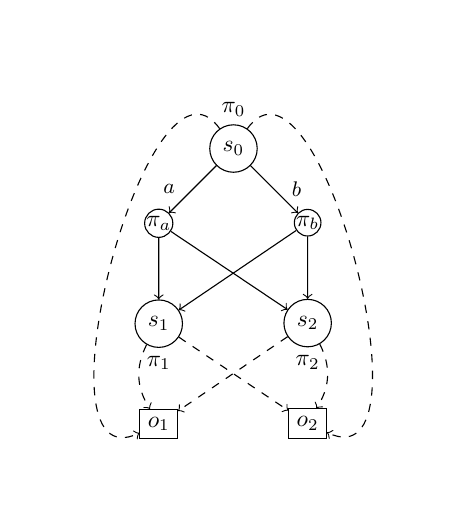
\begin{tikzpicture}[->, every node/.style={transform shape},node distance=1.5cm,thin, every path/.style={transform shape},scale=0.85,
	  node/.style={circle,transform shape,fill=white,draw,font=\sffamily},
	  dot/.style={shape=circle,transform shape,fill=white,draw,minimum size=4pt,inner sep=0pt},
	  obs/.style={rectangle,transform shape,fill=white,draw,font=\sffamily}]
	  \node[node] (0) [label=above:$\pi_0$,draw]{$s_0$};
	  \node[dot] (0a) [below left=1cm of 0] {$\pi_a$};
	  \node[dot] (0b) [below right=1cm of 0] {$\pi_b$};
	  \node[node] (1) [below of = 0a, label=below:$\pi_1$,draw] {$s_1$};
	  \node[node] (2) [below of = 0b, label=below:$\pi_2$,draw] {$s_2$};
	  \node[obs] (o1) [below of = 1] {$o_1$};
	  \node[obs] (o2) [below of = 2] {$o_2$};
%
	  \path[every node/.style={font=\sffamily\small}]
	    (0) edge node [left=4pt] {$a$} (0a)
	    (0) edge node [right=4pt] {$b$} (0b)
	    (0a) edge node [left=4pt] {} (1)
	    (0a) edge node [left=4pt] {} (2)
	    (0b) edge node [left=4pt] {} (1)
	    (0b) edge node [left=4pt] {} (2)
	    (0) edge [dashed, bend right = 130] node [right=1pt] {} (o1)
	    (0) edge [dashed, bend left = 130] node [right=1pt] {} (o2)
	    (1) edge [dashed, bend right] node [right=1pt] {} (o1)
	    (1) edge [dashed] node [right=1pt] {} (o2)
	    (2) edge [dashed] node [right=1pt] {} (o1)
	    (2) edge [dashed, bend left] node [right=1pt] {} (o2);
	\end{tikzpicture}
	\end{center}
	\vspace{-1cm}
	\caption{An example of POMDP}
	\label{fig:pomdp}
\end{wrapfigure}

%
% arrow notations
We write $s \xrightarrow{a} s'$ when $s$ may perform action $a$ and go into $s'$, i.e., $T(s,a)(s') > 0$.
% and $s \xrightarrow{a}$ means that there exists a state $s'$ such that $s \xrightarrow{a} s'$. We write $s \dashrightarrow o$ when, after a step, state $s$ may generate observation $o$, i.e., $Z(s)(o) > 0$. Again, we write $s \xrightarrow{a,o} s'$ when $s$ may perform action $a$, generate observation $o$ and go into $s'$, i.e., $s \xrightarrow{a} s' \wedge s \dashrightarrow o$.
%
% paths set
$Paths^\mathcal{P}$ contains infinite sequences $\pi$ of elements $\pi_i = (s,o,a) \in \mathcal{S} \times \mathcal{O} \times \mathcal{A}$ for $i \in [0..]$, such that $s_i \xrightarrow{a_i} s_{i+1}$, $Z(s_i)(o_i) > 0$.
%A path $\pi$ of $\mathcal{P}$ is a sequence $(s_0,o_0,a_0),(s_1,o_1,a_1)\dots \in (\mathcal{S}\times\mathcal{O}\times\mathcal{A})^\omega $ where $s_i \xrightarrow{a_i} s_{i+1}$, $Z(s_i)(o_i) > 0$ and $i \in [0..]$.
%Let $Paths^\mathcal{P}$ denote the set of all paths in $\mathcal{P}$. For a path $\pi = (s_0,o_0,a_0),(s_1,o_1,a_1)\dots \in Paths^\mathcal{P}$, let $\pi_s[i] = s_i$ denote the $(i+1)$st state, $\pi_o[i] = o_i$ denote the $(i+1)$st observation and $\pi_a[i] = a_i$ denote the $(i+1)$st action of $\pi$. $FPaths^\mathcal{P} = \{\pi[..n] \ |\ n \in \mathbb{N} \wedge \pi \in Paths^\mathcal{P}\}$ denotes the set of finite paths of $\mathcal{P}$, where $\pi[..n] = (s_0,o_0,a_0),(s_1,o_1,a_1)\dots(s_n,o_n,a_n)$ represents the prefix of $\pi$ of length $n+1$. 
%
% scheduler
We define a finite-memory scheduler over $\mathcal{P}$ as a function $\eta : \mathcal{B}_\mathcal{S} \times FPaths_{\mathcal{A},\mathcal{O}}^\mathcal{P} \rightarrow \mathcal{A}$ such that 
$$
\eta(b,\pi) = 
\begin{cases}
	\eta(b^{\pi_{i,\mathcal{A}},\pi_{i,\mathcal{O}}},\pi[1..]) & \text{if } |\pi| > 0 \\
	\eta(b) & \text{otherwise} \\
\end{cases}
$$ 
where $\eta(b)$ is a memoryless scheduler that maps belief states into choices $\eta:\mathcal{B}\rightarrow\mathcal{A}$. We use $Sched^\mathcal{P}$  to denote
%and $FSched^\mathcal{P}$ respectively 
the set of all (memoryless) 
%and finite-memory 
schedulers over \ac{POMDP} $\mathcal{P}$. 
%We use the term scheduler as a shortcut for memory-less scheduler.
% internal MDP
We use $\overline{\mathcal{P}} = \langle \mathcal{S}_\mathcal{P}, \mathcal{A}_\mathcal{P}, T_\mathcal{P} \rangle$ to isolate the hidden \ac{MDP} from the partially observable model.

% induced HMM
We can use a scheduler to solve choices of a \ac{POMDP}. When we apply a scheduler to a \ac{POMDP} in this way, we obtain a \ac{HMM} defined as follows

\begin{definition}[Induced \ac{HMM}]
	Let $\mathcal{P} = \langle \mathcal{S}, \mathcal{A}, T, \mathcal{O}, Z \rangle$ be a \ac{POMDP} and $\eta \in Sched(\overline{\mathcal{P}})$. The \ac{HMM} $\mathcal{P}_\eta$ is given by
	\vspace{-.3cm}
$$ \mathcal{P}_\eta = \langle \mathcal{S}, T_\eta, \mathcal{O}, Z \rangle $$

\vspace{-.3cm}
\noindent
where $T_\eta(s) = T(s,\eta(s))$ for every $s \in \mathcal{S}$.
\end{definition}

Given a belief state $b$ we can apply an action $a$ and an observation $o$ to compute the next belief state $b' = b^{a,o}$. We can compute such state, even considering the effect of a single action or a single observations, with the following belief update formulae

\begin{equation}\label{eq:belief_update_ao}
	b^{a,o}(s') = \frac{Z(s')(o)\sum_{s\in \mathcal{S}} T(s,a)(s')b(s)}{\sum_{\tilde{s}\in\mathcal{S}} Z(\tilde{s})(o)\sum_{s\in \mathcal{S}} T(s,a)(\tilde{s})b(s)}
\end{equation}
\begin{equation}\label{eq:belief_update_a}
	b^{a}(s') = \sum_{s\in \mathcal{S}} T(s,a)(s')b(s)
\end{equation}
%\begin{equation}\label{eq:belief_update_o}
%	b^{o}(s') = \frac{b(s') \cdot Z(s')(o)}{\sum_{s\in\mathcal{S}} b(s)\cdot Z(s)(o)}
%\end{equation}

%where $Pr(o|a,b) = \sum_{s'\in\mathcal{S}} Z(s')(o)\sum_{s\in \mathcal{S}} T(s,a)(s')b(s)$.

%\begin{definition}[\ac{BMDP}]
%Let $\mathcal{P} = \langle \mathcal{S}, \mathcal{A}, T, \mathcal{O}, Z \rangle$ be a \ac{POMDP}. %The \ac{BMDP} of $\mathcal{P}$ is given by the \ac{MDP} $\mathcal{M}(\mathcal{P}) = \langle \Delta(\%mathcal{S}), \mathcal{A}, T^\mathcal{M} \rangle$ where:
%$$ T^\mathcal{M}(b,a)(b') = \sum_{o \in \mathcal{O} : b^{a,o}=b'} \sum_{s' \in S} Z(s')(o) \sum_{s \%in S} b(s) \cdot T(s,a)(s') $$
%\end{definition}
%
%Given an observable history $h = (a_0,o_0),(a_1,o_1),\dots,(a_n,o_n) \in FPaths_\mathcal{O}^\mathcal{P}$ on a \ac{POMDP} $\mathcal{P}$ and an initial belief $b_0$, a \emph{belief path} on a \ac{BMDP} $\mathcal{M}(\mathcal{P})$ is a sequence $(b_0,a_0,o_0),(b_1,a_1,o_1),\dots,(b_n,a_n,o_n)$ where $b_{i+1} = b_i^{a_i,o_{i+1}}$. The set containing all the belief paths is denoted as $BPaths^\mathcal{P} \equiv FPaths^{\mathcal{M}(\mathcal{P})}$.

%We can write $b \xrightarrow{a} b'$ to say that $b' = b^{a,o}$, then we can also write a belief path as $b_0 \xrightarrow{a_0} b_1 \xrightarrow{a_1} b_2 \dots \xrightarrow{a_{n-1}} b_n$. % FIX non torna

% subsection partial_observability (end)

% section preliminaries (end)

%!TEX root = main.tex
\vspace{-.8cm}
\section{Methodology} % (fold)
\label{sec:model}

\begin{wrapfigure}[19]{r}{0.5\textwidth}
%\begin{figure}[H]
	\setlength{\abovecaptionskip}{-0.1em}
	\setlength{\belowcaptionskip}{-1em}
	\pgfdeclarelayer{background}
	\pgfdeclarelayer{foreground}
	\pgfsetlayers{background,main,foreground}
	\begin{tikzpicture} [
	   auto, scale=0.7, every node/.style={scale=0.7},
	   block/.style    = { rectangle, top color=white, bottom color=blue!30, 
	                            draw=blue!50!black!100, text width=6em, text centered, rounded corners, minimum height=2.5em },
	   line/.style     = { draw,thick,->,minimum height=1em },
	 ]
	  % Define nodes in a matrix
	  \matrix [column sep=1mm, row sep=3mm] {
	  	\node (pos1){}; &&&& \\
		&\node [block] (phase1){LTS}; & \node [block] (phase2){MDP}; & \node [block] (phase3){Observation function $Z$}; & \\
		&& \node [block] (phase4){POMDP}; && \\
		&& \node [block] (phase5){Explicit MDP}; & \node [block] (phase6) {LTL goal formula}; & \\
		&& \node (null2) {}; && \\
		&& \node [block] (phase7){Scheduler}; && \\
		&&&& \node (pos2){}; \\
		\node (pos3){}; && \node (null3){};&& \\
		&& \node [block] (phase8){Run-time choices}; && \\
		&&&& \node (pos4){}; \\
	 };

	 \node (mc) at (null2)[left=5pt] {\textit{model checking}};
	 \node (deploy) at (null3)[above left=1pt] {\textit{deploy}};

	  %\node [above,draw=gray!10, fit= (null1) (phase6), inner sep=0.1cm] {};
	 \begin{pgfonlayer}{foreground}
	 % connect all nodes defined above
	  \begin{scope} [every path/.style=line]
	%
		\path (phase1) |- (phase4);
		\path (phase2) -- (phase4);
		\path (phase3) |- (phase4);
	%
		\path (phase4) -- (phase5);
	%	
		\path (phase5) -- (phase7);
		\path (phase6) |- (null2);
	%
		\path (phase7) -- (phase8);
	%	\path (phase5) -- e [near start] {} (cvmpEnd);
	%	\path (phase5) -- e [near start] {} (cvmpEnd);
	%	\path (phase5) -- (phase6);
	%	\path (phase6) -- e [near start] {} (cvmpEnd);
	        %Recursions
	    %\path[dotted] (phase4)   --++  (-3,0) node{} |- (null1);
	   %\path[dotted] (phase6)   --++  (3,0) node{} |- (null1);
	 \end{scope}
	\end{pgfonlayer}

	\begin{pgfonlayer}{background}
	  	\path[fill=yellow!20,rounded corners, draw=black!50, dashed] (pos1) rectangle (pos2) node [above left=10pt, text=black!50] {OFF-LINE};
		\path[fill=yellow!20,rounded corners, draw=black!50, dashed] (pos3) rectangle (pos4) node [above left=10pt, text=black!50] {ON-LINE};
	\end{pgfonlayer}
	\end{tikzpicture}
	\caption{Elements and dependences of the proposed methodology}
	\label{fig:flow}
%\end{figure}
\end{wrapfigure}

In this section we define the necessary models by relying on the preliminary notions introduced in Section~\ref{sec:preliminaries} and show how these models can be transformed and used. The proposed methodology is depicted in Figure~\ref{fig:flow} where dependencies between components are shown.

We define a general framework to model a generic scenario that involves the controller of an adaptive agent and the surrounding environment.
The controller performs (output) actions and has neither uncertainties on state transitions nor uncertainties on state observations; it is a fully observable non probabilistic system that can be modeled as a \ac{LTS}. The agent performs (input) actions with uncertain state transitions, finally the environment is modeled as a \ac{MDP}. Partial observability is introduced later in this section to model what the adaptive agent perceives from the environment and in what measure.
%\setlength\intextsep{0pt}

We compose \ac{LTS} and \ac{MDP} together with an observation function that models what the agent perceives from the environment to obtain a \ac{POMDP} that describe the whole system. We get rid of incomplete information by transforming the partially observable model into another \ac{MDP} that transfers observations to states. Further more, we show that the properties verified on the new \ac{MDP} also holds for the previous model and we exploit this result to build a scheduler for the initial \ac{LTS}. The scheduler is computed in order to maximize the probability of satisfying a given goal, expressed as a \ac{LTL} formula that can refer to the agent's perceptions. Finally the scheduler is deployed on the agent that can take decisions at run-time.

Most of the workload is located in the model transformation phase, when the state space grows significantly. However the nature of the adaptation problem allow us to split the method into an off-line and an on-line phase: in the former the scheduler is built and provided to the agent that can use it during the latter phase. %Acceding to 
Determining the action to perform at run-time can be done in a very short time since the scheduler is a light data structure that maps the current configurations of local states and observations into actions.

\subsection{Composing agents models and their environment} % (fold)
\label{sub:composing_agents_models_and_their_environment}

%\marginpar{Non capisco. Eliminare fino ad actions.?}
Given a state, a \ac{LTS} describe what decision can be made by the agent.
%, that is free to choose any of the available actions. 
The following definition introduces the notion of \textit{compatibility} between an agent and its environment to guarantee communications without lost messages; the agent cannot do anything that the environment cannot perceive.

\begin{definition}[Compatibility]
We say that a \ac{LTS} $\mathcal{L}$ % = \langle \mathcal{S}_\mathcal{L}, \mathcal{A}_\mathcal{L}, T_\mathcal{L} \rangle$ 
and a \ac{MDP} $\mathcal{M}$ % = \langle \mathcal{S}_\mathcal{M}, \mathcal{A}_\mathcal{M}, T_\mathcal{M} \rangle$ 
are \emph{compatible} when $\mathcal{A}_\mathcal{L} \subseteq \mathcal{A}_\mathcal{M}$
\end{definition}

%We force further this concept, if compatibility express the possibility to receive a message from the agent, \textit{responsiveness} says that the environment cannot avoid to receive it, whatever its state is.

We push further this notion, to express the fact that the environment has to be \textit{responsive} and cannot avoid receiving messages from an agent.

\begin{definition}[$\mathcal{A}$-responsiveness]
Let $\mathcal{M}$ be a \ac{MDP} and $\mathcal{A} \subseteq \mathcal{A}_\mathcal{M}$. $\mathcal{M}$ is said \emph{$\mathcal{A}$-responsive} if
$$ \forall\ a\in \mathcal{A}, s\in \mathcal{S}_\mathcal{M}\ \exists\ s'\in \mathcal{S}_\mathcal{M}\ .\ T_\mathcal{M}(s,a)\neq \bot $$
\end{definition}

Responsiveness of the environment to agents actions ensures that communication between them is forced to happen at every step. 
%This property fits the situation in which the environment may always be affected by an agent action.

%We say that a \ac{POMDP} $\mathcal{P}$ is $\mathcal{A}$-responsive if the hidden \ac{MDP} $\overline{\mathcal{P}}$ is $\mathcal{A}$-responsive.

%\begin{definition}[Scheduler]
%	Let $\mathcal{P} = \langle \mathcal{S}, \mathcal{A}, T, \mathcal{O}, Z \rangle$ be an $\mathcal%{A}'$-responsive \ac{POMDP}, for $\mathcal{A}' \subseteq \mathcal{A}$. A \emph{memory-less %scheduler} for $\mathcal{P}$ is a function $\eta : \mathcal{B} \rightarrow \mathcal{A}'$.
%\end{definition}

%We denote with $Sched^\mathcal{P}$ the set of all the possible schedulers for $\mathcal{P}$.

\begin{definition}[Product \ac{POMDP}]
Let $\mathcal{L}$
%$ = \langle \mathcal{S}_\mathcal{L}, \mathcal{A}_\mathcal{L}, T_\mathcal{L} \rangle$ 
be a \ac{LTS}, $\mathcal{M}$
%$ = \langle \mathcal{S}_\mathcal{M}, \mathcal{A}_\mathcal{M}, T_\mathcal{M} \rangle$ 
be a \ac{MDP} such that 
%$\mathcal{L}$ and $\mathcal{M}$ are \emph{compatible} and 
$\mathcal{M}$ is $\mathcal{A}_\mathcal{L}$-\emph{responsive}, and let $Z : \mathcal{S}_\mathcal{L} \times \mathcal{S}_\mathcal{M} \rightarrow \Delta(\mathcal{O})$ be an observation function with codomain in an observation set $\mathcal{O}$. We call the composition of the system a \it{product} \ac{POMDP} that is defined as the following \ac{POMDP}
$$ \mathcal{W} (\mathcal{L},\mathcal{M},Z,\mathcal{O}) = \langle \mathcal{S}_\mathcal{L} \times \mathcal{S}_\mathcal{M}, \mathcal{A}_\mathcal{L}, T_\mathcal{W}, \mathcal{O}, Z \rangle$$
where the transition function $T_\mathcal{W} : \mathcal{S}_\mathcal{L} \times \mathcal{S}_\mathcal{M} \times \mathcal{A}_\mathcal{L} \rightarrow \Delta(\mathcal{S}_\mathcal{L} \times \mathcal{S}_\mathcal{M})$ is defined as follows
$$ T_\mathcal{W}(s_l,s_m,a_l)(s_l',s_m') = \begin{cases}
T_\mathcal{M}(s_m,a_l)(s_m') \quad \text{if } s_l\xrightarrow{a_l}_\mathcal{L}s_l' \\ %\wedge s_m \xrightarrow{a_l}_\mathcal{M} s_m' \\
0 \quad \text{otherwise}
\end{cases}$$
\end{definition}

Once the communication between agent and environment is correctly defined, we can safely compose the two elements into a product \ac{POMDP} that represents their synchronized progress. The state contains now local and environmental information, the former are assumed to be known while the latter are not. 
%However this pair of states determines how the observations are likely. 

%\marginpar{Current state construction}
If we know
%we assume to have
the current state for both the components, say $l \in \mathcal{S}_\mathcal{L}$ a state of $\mathcal{L}$ and $m \in \Delta(\mathcal{S}_\mathcal{M})$ a belief state of $\mathcal{M}$, we can build the corresponding belief state $b_{\mathcal{W}} \in \mathcal{B}_\mathcal{W}$ of the product \ac{POMDP} as the following function $b_\mathcal{W} : \mathcal{S}_\mathcal{L} \times \Delta(\mathcal{S}_\mathcal{M}) \rightarrow \Delta(\mathcal{S}_\mathcal{L}\times \mathcal{S}_\mathcal{M})$
\begin{equation*}
b_\mathcal{W}(s,b)(l,m) =  
\begin{cases}
	b(m) & \text{if } l = s \\
	0 & \text{otherwise} \\
\end{cases}
\end{equation*}
%
We can then obtain the initial belief state of $\mathcal{W}$ as $b_{\mathcal{W}}(s_0,b_0)$, where $s_0$ is the initial state of $\mathcal{L}$ and $b_0$ is the initial belief state of $\mathcal{M}$.

\begin{example}\label{ex:pomdp}
We can merge the controller of Example~\ref{ex:controller} with the environment of Example~\ref{ex:environment} to obtain a \ac{POMDP}.
To compute this \ac{POMDP} we need to define how the main robot perceives the others. 
We assume that the robot can perceive the presence of at least one robot in each of the four adjacent positions or in its own position, and that this perception is not affected by precision errors. 
%For sake of simplicity we consider the function $around(x,y)$ that returns the set of positions immediately next to $(x,y)$ and the local position itself. 
Starting from a set of basic observations $ basic = \left\{north, south, east, west, here \right\} $ we obtain the set of possible observations as the power set $\mathcal{O} = 2^{basic}$, indeed every basic observation can happen independently from the others. $next(s_0,o)$, where $s_0$ is the position of the white robot and $o$ is a basic observation, is used to represent the position perceived by sensors. The observation function can be then defined in the following way
$$
\begin{array}{rcl}
	Z(s_0,s_1,s_2)(O) &=& 
	\begin{cases}
		1 & \text{if } s_1 = next(s_0,o) \vee s_2 = next(s_0,o), \ \forall\ o \in O \\
		0 & \text{otherwise} \\
	\end{cases} \\[.5cm]
\end{array}
$$

\vspace{-.3cm}
\qed
\end{example}

%\marginpar{Scheduler construction}
We exploit the construction of the \ac{POMDP} $\mathcal{P}$ starting from an \ac{LTS} $\mathcal{L}$ to drive the possible sequence of choices. Let $\eta \in Sched^\mathcal{L}$ be a scheduler and let $\sigma = \eta(s_0),\eta(s_1),\eta(s_2),\dots$ be the sequence of actions induced by $\eta$, where $s_i = T_\mathcal{L}(s_{i-1},\eta(s_{i-1}))$ for $i \in \mathbb{N}$. We can then construct a scheduler $\overline\eta$ for a product \ac{POMDP} $\mathcal{W}$ as a function $\overline\eta : \mathcal{S}_\mathcal{L} \times \Delta(\mathcal{S}_\mathcal{M}) \rightarrow \mathcal{A}_\mathcal{L}$ such that $ \overline\eta(l,b) \in init(l) $. We denote the set of this kind of schedulers as $Sched^\mathcal{W}$. 
%, where $s_0 \in \mathcal{S}_\mathcal{L}$ and $b_0 \in \Delta(\mathcal{S}_\mathcal{M})$ are respectively the initial state of $\mathcal{L}$ and the initial belief state of $\mathcal{M}$.

%\marginpar{Scheduler sets equivalence}
We are able to show that the set of schedulers on $\mathcal{L}$ and the set of schedulers extended to $\mathcal{W}$ are essentially the same since every scheduler preserves the induced sequence of actions after the extension. This is due to the fact that extended schedulers act only on the projection of $\mathcal{W}$ on $\mathcal{L}$.

\begin{proposition}\label{prop:sched}
Let $\mathcal{W}(\mathcal{L},\mathcal{M},Z,\mathcal{O})$ be a product \ac{POMDP}, $\eta \in Sched^\mathcal{L}$, then $\forall\ s \in \mathcal{S}_\mathcal{L}$ and $\forall\ a \in \mathcal{A}_\mathcal{L}$ 
%$$ \eta(s) = a \iff \overline\eta(s,b) = a $$
$$ T_\mathcal{L}(s,\eta(s)) = s' \iff \sum_{m \in \mathcal{S}_\mathcal{M}} T_\mathcal{W}(s,\cdot,\overline\eta(s,\cdot))(s',m) = 1 $$
\end{proposition}

%\marginpar{Always known choices}
The following result says that belief states of $\mathcal{W}(\mathcal{L}, \mathcal{M}, Z, \mathcal{O})$ that give probability mass to a single state in $\mathcal{S}_\mathcal{L}$ will transfer all the probability only to states containing the successive state of $\mathcal{L}$. This means that if the local state is known at the current time, it will be known even after an action execution.

\begin{proposition} \label{prop:beliefprob}
Let $\mathcal{W}(\mathcal{L},\mathcal{M},Z,\mathcal{O})$ be a product \ac{POMDP}, $l,l' \in \mathcal{S}_\mathcal{L}$, $b \in \mathcal{B}_\mathcal{W}$ and $\exists\ a \in \mathcal{A}_\mathcal{L} : l \xrightarrow{a} l'$, then 
$$ \sum_{m \in \mathcal{S}_{\mathcal{M}}} b(l,m) = 1 \Rightarrow \sum_{m\in \mathcal{S}_{\mathcal{M}}} b^{a,o}(l',m) = 1 $$
\end{proposition}

%Given a \ac{POMDP} we can build an equivalent \ac{MDP} that can be used to compute the probability of reaching the expected goal. Note that, thanks to this translation, we can use standard and well known tools to perform analysis of a \ac{POMDP}.

We define now the transformation of a \ac{POMDP} into a fully observable \ac{MDP}.The transformation does preserve some information of the probability measure that makes it possible to convert some model checking results on the \ac{MDP} to valid results on the \ac{POMDP}.

% explicit MDP
\begin{definition}[Explicit Markov decision process]\label{def:emdp}
Let $\mathcal{P} = \langle \mathcal{S},\mathcal{A},T,\mathcal{O},Z \rangle$ be a \ac{POMDP}, we define the \emph{explicit \ac{MDP}} $\widehat{\mathcal{P}}$ of $\mathcal{P}$ as the following \ac{MDP}
$$ \widehat{\mathcal{P}} = \langle \mathcal{S}\times\mathcal{O}, \mathcal{A}, \widehat{T}, \mathscr{L} \rangle $$
where 
\begin{itemize}
	\item $\widehat{T}((s,o),a)(s',o') = T(s,a)(s')\cdot Z(s')(o')$
	\item $\mathscr{L}(s,o) = o$
\end{itemize}
\end{definition}
%
\setlength\intextsep{0pt}
\begin{wrapfigure}{r}{0.45\textwidth}
	\begin{center}
	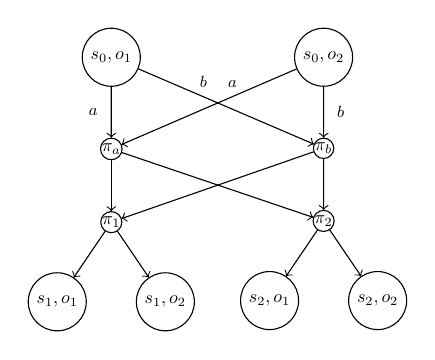
\begin{tikzpicture}[->, every node/.style={transform shape},node distance=1.5cm,thin, every path/.style={transform shape},scale=0.65, node/.style={circle,transform shape,fill=white,draw,font=\sffamily}, dot/.style={shape=circle,transform shape,fill=white,draw,minimum size=4pt, inner sep=0pt}]
%	  \node[node] (init) [label=below:$\pi_0$,draw]{init};
%	  \node[node] (s0o1) [below left = 1cm and 1.5cm of init] {$s_0,o_1$};
%	  \node[node] (s0o2) [below right = 1cm and 1.5cm of init] {$s_0,o_2$};
	  \node[node] (s0o1) {$s_0,o_1$};
	  \node[node] (s0o2) [right = 3cm of s0o1] {$s_0,o_2$};
	  \node[dot] (pa) [below = 1cm of s0o1] {$\pi_a$};
	  \node[dot] (pb) [below = 1cm of s0o2] {$\pi_b$};
	  \node[dot] (p1) [below = 1cm of pa] {$\pi_1$};
	  \node[dot] (p2) [below = 1cm of pb] {$\pi_2$};
	  \node[node] (s1o1) [below left = 1cm and 0.5cm of p1] {$s_1,o_1$};
	  \node[node] (s1o2) [below right = 1cm and 0.5cm of p1] {$s_1,o_2$};
	  \node[node] (s2o1) [below left = 1cm and 0.5cm of p2] {$s_2,o_1$};
	  \node[node] (s2o2) [below right = 1cm and 0.5cm of p2] {$s_2,o_2$};
	  
	  \path[every node/.style={font=\sffamily\small}]
%	    (init) edge node {} (s0o1)
%	    (init) edge node {} (s0o2)
		
	    (s0o1) edge node [left=4pt] {$a$} (pa)
	    (s0o1) edge node [above left=10pt] {$b$} (pb)

	    (s0o2) edge node [above right=10pt] {$a$} (pa)
	    (s0o2) edge node [right=4pt] {$b$} (pb)

	    (pa) edge node {} (p1)
	    (pa) edge node {} (p2)

	    (pb) edge node {} (p1)
	    (pb) edge node {} (p2)
		
		(p1) edge node {} (s1o1)
		(p1) edge node {} (s1o2)
		
		(p2) edge node {} (s2o1)
		(p2) edge node {} (s2o2);
		
	\end{tikzpicture}
	\end{center}
	\caption{Explicit \ac{MDP} of the \ac{POMDP} in Figure~\ref{fig:pomdp}}
	\label{fig:explicitmdp}
%\end{figure}
\end{wrapfigure}
The \ac{POMDP} model is transformed into an \ac{MDP} considering observations as atomic propositions of the new states, indeed we consider perceptions as part of the state and we modify the probability weights on transitions in order to preserve %how likely it is to end
the likelihood of ending up into a state and make a specific observation. 

An example of transformation is depicted in Figure~\ref{fig:explicitmdp}, big circles are states, small circles are distributions, rectangles are observations, arrows are transitions and dashed arrows are observation distributions. The explicit \ac{MDP} has two levels of distributions that represents a product distribution between the transition function and the observation function. During the transformation, we lose information about the observation made in the initial state, this loss will be taken into account when constructing the scheduler.

% subsection composing_agents_models_and_their_environment (end)
\vspace{-.3cm}
\subsection{Specifying agents goals} % (fold)
\label{sub:specify_agents_goals}

The last ingredient of our approach is the language used to describe the required and expected goals. In this context we will use \ac{LTL} formulae specialized to handle \ac{POMDP}, indeed the syntax (and consequently the satisfaction relation) of this logic differs from the classical one only for the presence of an observation as a terminal, instead of a set of atomic propositions.

\begin{definition}[Syntax of \ac{LTL}]
A \ac{LTL} formula $\varphi$ is defined as follows
$$ \varphi ::= tt\ |\ o\ |\ \varphi_1 \wedge \varphi_2\ |\ \neg\varphi\ |\ \bigcirc \varphi\ |\ \varphi_1 U \varphi_2 $$
where $o \in \mathcal{O}$.
\end{definition}

Let $LTL$ denote the set of all possible \ac{LTL} formula. We define the satisfaction relation $\models$ with respect to a \ac{HMM} $\mathcal{H}$ by induction in the following way

\begin{definition}[Satisfaction relation]
The satisfaction relation $\models\ \subseteq Paths_\mathcal{O}^\mathcal{H}\times LTL$ is defined by induction as follows:
$$
\begin{array}{lll}
	\pi \models tt & & \text{always} \\
	\pi \models o & \text{ iff } & \pi_0 = o \\
	\pi \models \varphi_1 \wedge \varphi_2 & \text{ iff } & \pi \models \varphi_1 \wedge \pi \models \varphi_2 \\
	\pi \models \neg \varphi & \text{ iff } & \pi \not\models \varphi \\
	\pi \models \bigcirc \varphi & \text{ iff } & \pi[1..] \models \varphi \\
	\pi \models \varphi_1 U \varphi_2 & \text{ iff } & (\exists\ i \in [0..]\ .\ \pi[i] \models \varphi_2 \wedge \forall\ j \in [0..i-1]\ \pi[j] \models \varphi_1) \\
	&& \quad \vee\ \forall\ k \in \mathbb{N}\ .\ \pi[k] \models \varphi_1 \\
\end{array}
$$
\end{definition}

This logic is employed to express desired behaviour for the adaptive agent, like liveness, safety or time bonded properties of signals coming from the environment.

\begin{example}\label{ex:formula}
The problem of avoiding collisions with other robots as addressed with the following \ac{LTL} formula
$$ \varphi_{avoid} = \neg\ collision \wedge \bigcirc \neg\ collision $$
%$$ Pmin=?[ G<=1 (! "collision")] $$
where label $collision$ is defined as $\bigvee_{o \in \mathcal{O} : here \in o}o$.
\end{example}

Let $\mathcal{M}$ be a \ac{MDP}. For any formula $\varphi \in LTL$ and for any initial state $s \in \mathcal{S}_\mathcal{M}$, we define the following probability measure ($\models^*$ is the satisfaction relation defined for the classical \ac{LTL}, see~\cite[Definition 5.7]{Katoen-Baier})
%\begin{equation}\label{eq:pmax}
%p_{max}^\mathcal{P}(s,\varphi) \triangleq \sup_{\eta \in Sched^\mathcal{P}} \left(Pr_s^{\mathcal{P}_\eta}\{\pi \in Paths_\mathcal{O}^{\mathcal{P}_\eta}\ |\ \pi \models \varphi \}\right)
%\end{equation}
\begin{equation}\label{eq:pmin_mdp}
p_{min}^\mathcal{M}(s,\varphi) \triangleq \inf_{\eta \in Sched^\mathcal{M}} \left(Pr_s^{\mathcal{M}_\eta}\{\pi \in Paths^{\mathcal{M}_\eta}\ |\ \pi \models^* \varphi \}\right)	
\end{equation}

Let $\mathcal{P}$ be a \ac{POMDP}. For any formula $\varphi \in LTL$ and for any initial state $s \in \mathcal{S}_\mathcal{P}$, we define the following probability measure
%\begin{equation}\label{eq:pmax}
%p_{max}^\mathcal{P}(s,\varphi) \triangleq \sup_{\eta \in Sched^\mathcal{P}} \left(Pr_s^{\mathcal{P}_\eta}\{\pi \in Paths_\mathcal{O}^{\mathcal{P}_\eta}\ |\ \pi \models \varphi \}\right)
%\end{equation}
\begin{equation}\label{eq:pmin}
p_{min}^\mathcal{P}(s,\varphi) \triangleq \inf_{\eta \in Sched^\mathcal{P}} \left(Pr_s^{\mathcal{P}_\eta}\{\pi \in Paths_\mathcal{O}^{\mathcal{P}_\eta}\ |\ \pi \models \varphi \}\right)	
\end{equation}

%We can easily generalize equations~(\ref{eq:pmax}) and~(\ref{eq:pmin}) to belief states by $Pr_b(C) = \sum_{s\in\mathcal{S}}b(s)\cdot Pr_s(C)$.

%We define the probability measure extended to belief states as a discrete random variable to preserve the probabilistic weight of every single case of minimum probability obtained by an initial state. These kind of information would be lost if we considered a minimum probability over belief states defined as the average $p^\mathcal{P}_{min}(b,\varphi) = \sum_{s\in\mathcal{S}}b(s)\cdot p_{min}^\mathcal{P}(s,\varphi)$. The definition is then the following
%\begin{equation}\label{eq:pminb}
%p_{min}^\mathcal{P}(b,\varphi) \triangleq \min_{s \in \mathcal{S}} b(s)\cdot p_{min}^\mathcal{P}(s,\varphi)
%\end{equation}
%where $\min$ is the aggregation function over $\mathcal{S}$ instead of $\sum$.

The following result allows to compute the minimum probability of satisfying a formula $\varphi$ on a \ac{POMDP} by 
%means of aggregation of 
aggregating the
minimum probabilities computed on the respective explicit \ac{MDP}, recovering the initial observation probabilities lost during the model transformation.

\begin{theorem}\label{teo:pmins}
Let $\mathcal{P}$ be a \ac{POMDP}, $\widehat{\mathcal{P}}$ the explicit \ac{MDP} of $\mathcal{P}$, $\varphi$ an LTL formula with $AP = \mathcal{O}$, then it holds
%	$$ p_{min}^\mathcal{P}(s, \varphi) = \min_\eta Pr_s^{\mathcal{P}_\eta}\{\pi \in (\mathcal{S}\times\mathcal{O})^\omega\ |\ \pi \models \varphi\} $$
	$$ p_{min}^\mathcal{P}(s, \varphi) \leq \sum_{o\in\mathcal{O}} Z_\mathcal{P}(s)(o) \cdot p_{min}^{\widehat{\mathcal{P}}}((s,o), \varphi) $$
\end{theorem}

The converse inequality holds for the maximum probability.

%The result cannot be extended to belief states, in general it only holds
%\begin{equation} 
%p_{min}^\mathcal{P}(b,\varphi) \geq \sum_{s \in \mathcal{S}}b(s)\sum_{o \in \mathcal{O}} Z(s)(o) \%cdot p_{min}^{\widehat{\mathcal{P}}}((s,o),\varphi)
%\end{equation}
%because of the case in which $b(l,m) > 0$ and $b(l,m') > 0$

\begin{corollary}\label{cor:infmin}
Let $\mathcal{P}$ be a \ac{POMDP}, $s \in \mathcal{S}_{\mathcal{P}}$ and $\varphi \in LTL$, it holds
$$ p_{min}^\mathcal{P}(s,\varphi) = \min_{\eta\in Sched^\mathcal{P}} \left(Pr_s^{\mathcal{P}_\eta}\{\pi \in Paths_\mathcal{O}^{\mathcal{P}_\eta}\ |\ \pi \models \varphi \}\right) $$
\end{corollary}

%We introduce the concept of \emph{entry point} of an explicit \ac{MDP}: an entry point is a %fictitious state $s_{new}$ that simulate the initial belief state.
%
%\begin{definition}[Entry point]
%	Let $\mathcal{W} = \langle \mathcal{L}, \mathcal{M}, Z \rangle$ be a product \ac{POMDP}, $b \in %\Delta(\mathcal{S}_\mathcal{L}\times\mathcal{S}_\mathcal{M})$ a belief state and $\widehat{\%mathcal{W}}$ an explicit \ac{MDP} then $\widehat{\mathcal{W}}_b$ is defined as the following \ac%{MDP}
%	$$ \widehat{\mathcal{W}}_{b} = \langle (\mathcal{S}\times\mathcal{O}) \cup \{s_{new}\}, \mathcal%{A}\cup\{\tau\}, \widehat{T}, \mathscr{L} \rangle $$
%where $\widehat{T}(s_{new},\tau)(s,o) = b(s)\cdot Z(s)(o)$, $\mathscr{L}(s_{new}) = \bot$ %and the rest remains unchanged.
%\end{definition}
%
%\begin{proposition}
%$$ p_{min}^\mathcal{P}(b,\varphi) = p_{min}^{\widehat{\mathcal{P}}_b} (s_{new},\bigcirc \varphi) $$
%\end{proposition}

Now we can use 
%the result achieved in 
Theorem~\ref{teo:pmins} to define the value function that will be used as optimization criterion from the scheduler. Since we need to evaluate the effect of actions executed from a belief state, we need another level of aggregation; we thus choose to maximize the average of the minimum probabilities weighted on belief probabilities.

\begin{definition}[Value function]
Let $\mathcal{W}(\mathcal{L},\mathcal{M},Z,\mathcal{O})$ be a product \ac{POMDP}, the value function of $\mathcal{W}$ of a belief state $b\in\mathcal{B}$ and an action $a\in\mathcal{A}_\mathcal{L}$ with respect to an \ac{LTL} formula $\varphi$ is defined as follows
$$ V_a^\mathcal{W}(b,\varphi)= \sum_{s\in\mathcal{S}} b^a(s)\cdot \sum_{o\in\mathcal{O}} Z(s)(o)\cdot p_{min}^{\widehat{\mathcal{W}}}((s,o),\varphi) $$
The scheduler $\mathfrak{S} \in Sched^\mathcal{W}$ is consequently defined as
$$ \mathfrak{S}_\varphi(b) = \argmax_{a\in\mathcal{A}_\mathcal{L}} V_a^\mathcal{W}(b,\varphi) $$
\end{definition}

% subsection specify_agents_goals (end)

%\marginpar{Random variable}
%We model these concepts as a random variable in the following way: the sample space $\Omega = \%mathcal{S}_\mathcal{W}$ is the state set of a \ac{POMDP} and the discrete random variable $X_\varphi%^\mathcal{W}$ is defined upon it as $X_\varphi^\mathcal{W}(s) = p_{min}^\mathcal{W}(s\models\varphi)%$. Consequently we can define the probability mass function as $f_X(s) = b(s)$ where $b$ represents %the initial belief state of the \ac{POMDP}. We have then 
%$$E[X] = \sum_{s \in \mathcal{S}} f_X(s) \cdot X(s) = \sum_{s \in \mathcal{S}} b(s) \cdot p_{min}^\%mathcal{W}(s\models\varphi) $$
%$$VAR[X] = E[(X-\mu)^2] = \sum_{s \in \mathcal{S}} f_X(s) \cdot \left(X(s) - \mu\right) = \sum_{s \%in \mathcal{S}} b(s) \cdot \left(p_{min}^\mathcal{W}(s\models\varphi) - \mu\right)$$


% section model (end)

%!TEX root = main.tex
\vspace{-1cm}
\subsection{Taking decisions} % (fold)
\label{sub:algorithm}

With Algorithm~\ref{alg:main} we define the on-line procedure used at every step to select the best action to execute. The algorithm consists in evaluating the value function $V_a^\mathcal{W}$ of every action considering the current belief state $b$. This is implemented by the cycle (lines $1-4$). 

At line $2$ we generate the belief state after an action $a$ using Equation~(\ref{eq:belief_update_a}). Equation~(\ref{eq:belief_update_a}) computes $b^a(s)$ in $O(|\mathcal{S}|^2)$, then we can obtain the entire state $b^a$ in $O(|\mathcal{S}|^3)$. The step at line $3$ is the
average over the minimum probabilities to satisfy $\varphi$ weighted by the probability of being in that state according to $b^a$. Computing $p^\mathcal{W}_{min}(s,\varphi)$ costs $O(k |\mathcal{O}| |\mathcal{S}|(|\mathcal{S}|+M))$ (see \cite[Theorem 10.127]{Katoen-Baier}) where $k$ is number of maximal end components of the composition of the \ac{MDP} with the \ac{DRA} representing the LTL formula $\varphi$, and $M$ is the number of triples $(s,a,s')$ such that $T(s,a)(s') > 0$. Summing everything up we can compute $V_{a}^\mathcal{W}$ in $O(k|\mathcal{O}||\mathcal{S}|^2(|\mathcal{S}|+M))$ that is polynomial and slightly dominates the complexity of $\textsc{Expand}(b,a)$. However we can precompute minimum probabilities in order to access them at execution time in $O(|\mathcal{S}|)$.

The construction of the \ac{DRA} $\mathcal{A}_\varphi$ is the most expensive operation in terms of computational complexity (2EXPTIME on $|\varphi|$). However this high complexity is not completely a bad news, indeed in linear time model checking we usually have short formulae and we can expect to have the same situation for planning. Moreover $\varphi$ does not change during the evaluation of every action, then it can be computed off-line once and for all the duration of the execution.

The last step, at line $5$, is just a search for the index of a maximum that has cost $O(|\mathcal{A}_\mathcal{L}|)$. %, that is irrelevant with respect to the complexity of the $for$ cycle $O(k|\mathcal{A}_\mathcal{L}||\mathcal{O}||\mathcal{S}|^2(|\mathcal{S}|+M))$ (lines $1-4$).
Considering precomputed minimum probabilities we have the following result

\begin{proposition}
Algorithm~\ref{alg:main} has complexity 
$O(|\mathcal{A}_\mathcal{L}||\mathcal{S}_\mathcal{W}|^2)$
%$O(k|\mathcal{A}_\mathcal{L}||\mathcal{O}|poly(size(\overline{\mathcal{W}})))$
\end{proposition}

\begin{algorithm}
	\SetKwInOut{Input}{input}
	\SetKwInOut{Output}{output}
	\Input{$\varphi \in \text{LTL}$, $b \in \mathcal{B}$, $\mathcal{W}\ \text{POMDP}$}
	\Output{$a_t \in \mathcal{A}_\mathcal{L}$}
	\For{$a \in \mathcal{A}_\mathcal{L}$}{
		$b^a \leftarrow \textsc{Expand}(b,a)$\;
		$V_{a}^\mathcal{W} \leftarrow \sum_{s\in\mathcal{S}} b^a(s) \cdot p_{min}^\mathcal{W}(s,\varphi)$\; % \sum_{o\in \mathcal{O}} Z(s,o) \cdot p_{min}^{\widehat{\mathcal{W}}}((s,o),\varphi)$\;
	}
	$a_t \leftarrow \argmax_{a \in \mathcal{A}_\mathcal{L}}V_{a}^\mathcal{W}$\;
	\Return{$a$\;}
 \caption{Online decision algorithm to compute $\mathfrak{S}_\varphi^\mathcal{W}(b)$}\label{alg:main}
\end{algorithm}


%!TEX root = main.tex
\vspace{-.3cm}
\section{Our approach at work} % (fold)
\label{sec:case_studies}

In this section we discuss the case study gradually introduced in Figure~\ref{fig:arenarobot} and in Examples \ref{ex:controller}, \ref{ex:dtmc}, \ref{ex:environment}, \ref{ex:pomdp} and \ref{ex:formula} where we described the controller of the black robot, the environment model composed by white robots, the merged model as a \ac{POMDP}, and a possible target formula $\varphi_{avoid}$.
%We model the arena as a square matrix and the status of every robot as its position using coordinates. We are interested in evaluating the behaviour produced by our scheduler considering different objective properties.

%\marginpar{LTS}
%The controller is modeled by a \ac{LTS} $\mathcal{L}$ and, since we are assuming that the controller is aware of its own position inside the arena, we can model the state as the couple of coordinates given by its position $(x_0,y_0)$. In general we put every known information inside the controller's status. We let the robot moves in any direction from any position, that means that the controller can always choose to go towards any direction (north, south, east, west or to stand still) and the next state will depend on the chosen action and the starting state. 

%We denote the dimension of the arena with $DIM$ that represent the number of rows or column of the matrix. States and actions of the controller are defined as follows
%$$
%\begin{array}{rcl}
%	\mathcal{S}_\mathcal{L} &=& \left\{ (x,y)\ |\ x,y = 1,\dots,DIM \right\} \\
%	\mathcal{A}_\mathcal{L} &=& \left\{ north, south, east, west, here \right\}	\\
%\end{array}
%$$
%and $n$, $s$, $e$, $w$, $h$ are for, respectively, north, south, east, west and here. 

%To ease the next definitions we say that the function $next(x,y,a)$ returns the position that we obtain starting from $(x,y)$ and applying direction $a \in \mathcal{A}_{\mathcal{L}}$, assuming that moving towards a wall will not change the current position. The transition relation can be defined then as $T_{\mathcal{L}}(s,a)= step(s,a)$
%The transition relation $T_\mathcal{L}$ is built in order to move the position in the given action, e.g., $T((x,y),west) = (x-1,y)$ if $x > 0$, $T_\mathcal{L}((x,y),west) = (x,y)$ otherwise.

%\marginpar{MDP}
%The environment is modeled by $\mathcal{M}$, a \ac{MDP} that represents the probabilistic behaviour of two other robots. They can move independently in the four directions or stand still as the main robot. We assume that their movement are fully probabilistic with a uniform distribution over the reachable positions. The state of the environment \ac{MDP} $M$ is then represented by the coordinates of the two robots ($\mathcal{S}_\mathcal{M} = \mathcal{S}_\mathcal{L}^2)$, and it can receive any action from the controller ($\mathcal{A}_\mathcal{M} = \mathcal{A}_\mathcal{L}$).

%The transition relation $T_\mathcal{M}$ can always accept any action from the controller, since it is completely reactive, and the probabilistic behaviour that follows is not influenced, in this specific case study, by this choice. The next state distribution is obtained as the product of the distributions of both the robots of the environment. Then we can define $ T_{\mathcal{M}}((s_1,s_2),\cdot)(s_1',s_2') = p $ where $s_1'$ and $s_2'$ are positions directly reachable by one step starting from $s_1$ and $s_2$ respectively. The probability $p$ is the same per every reachable state of $\mathcal{M}$.

%\marginpar{POMDP}
%To merge together controller and environment into a product \ac{POMDP} $\mathcal{W}(\mathcal{L},\mathcal{M},\mathcal{O},Z)$ we need to define how the main robot perceive the others. We assume that the robot can perceive the presence of at least one robot in each of the four adjacent positions or in its own position, and that this perception is not affected by precision errors. Starting from a set of basic observations $ basic = \left\{north, south, east, west, here \right\} $ we obtain the set of possible observations as the power set $\mathcal{O} = \mathcal{P}(basic)$, indeed every basic observation can happen independently from the others.
%$$
%\begin{array}{rcl}
%	Z(s_0,s_1,s_2)(\{o_1,\dots,o_n\}) &=& 
%	\begin{cases}
%		1 \quad \text{if } s_1 \in next(s_0,o_i) \wedge s_2 \in next(s_0,o_i) \ \forall\ i \\
%		0 \quad \text{otherwise} \\
%	\end{cases} \\[.5cm]
%\end{array}
%$$

%$\mathcal{W}$ describe the whole system. We convert it into the explicit \ac{MDP} $\widehat{\mathcal{W}}$ and we export it to the \texttt{PRISM} model checker~\cite{KwiatkowskaNP11} to compute the minimum probability of satisfying a given objective formula $\varphi$. We obtain then a minimum probability for every state of the system, in this case one for each disposition of the robots.

%The problem of avoiding collisions with other robots as addressed with the following \ac{LTL} formula
%$$ \varphi_{avoid} = \neg\ collision \wedge \bigcirc\ \neg\ collision $$
%$$ Pmin=?[ G<=1 (! "collision")] $$
%where label $collision$ is defined as $\bigvee_{o \in \mathcal{O} : here \in o}o$.

We have run some experiments to compare the criterion we adopted with other possible approaches. The \textsc{avg} scheduler, the one we propose, chooses the action which maximize the minimum probability averaged over the belief probabilities. With scheduler \textsc{max} we consider to maximize the maximum minimum probability weighted again with belief probabilities. The \textsc{rnd} scheduler makes the robot move towards a uniformly random direction that is not already taken by another robot. \textsc{rpl} is the repulsive approach: the robot stands still until he perceive another robot, then it starts to move to the opposite direction, without keeping any memory of the past. \textsc{rpl} is defined for each pair state-observation.

We compare all the different approaches in a $5 \times 5$ arena with three robots, running $100$ simulations for $100$ steps for each case. Every run starts from a random initial state. The experiments results are shown in Figure~\ref{fig:exp} (left-hand side) where we measure the cumulate number of collisions over time, summing up over all the runs. 

Apart from some specific situation with the highest density of robots, the \textsc{avg} scheduler 
%manage to avoid collisions and it 
behaves generally better with respect to the other schedulers for collisions avoidance. It is worth noting that, the higher is the arena, the lower is the density of robots inside it; then avoiding collisions becomes easier. The \textsc{max} scheduler turns out to be suitable only for some specific situations since it gets good performances with a high density of robots.
% but they decrease as the density decreases.

Keeping other robots under observation is another possible target that can be expressed with a \ac{LTL} formula in the following way:
\vspace{-.2cm}
$$ \varphi_{track} = \neg\ collision \wedge vision \wedge \bigcirc\ (\neg\ collision \wedge vision) $$

\vspace{-.2cm}
\noindent
where $vision$ is a label that stands for $\neg\ \varnothing$ meaning that the robot is perceiving ``nothing''. 
Results from simulations depicted in Figure~\ref{fig:exp} (right-hand side) are obtained with the same set up of the previous experiment, and show that the synthesized behaviour is such that the number of perceptions is maximized while the number of collisions is minimized. 
It is worth noting that, by considering closely the simulation it is possible to appreciate some counterintuitive movement pattern such as moving towards other robots:
%By watching closely to the simulation
%\marginpar{Come fanno a watch-arlo?}
%it is possible to notice some unintuitive movement pattern such as moving towards other robots: 
this behaviour is actually the one that maximize our target since the other robot is more likely to move away from its current position making room for the controlled robot and, at the same time, remaining in its sight with probability $1$.
\begin{figure}[htbp]
	\centering
	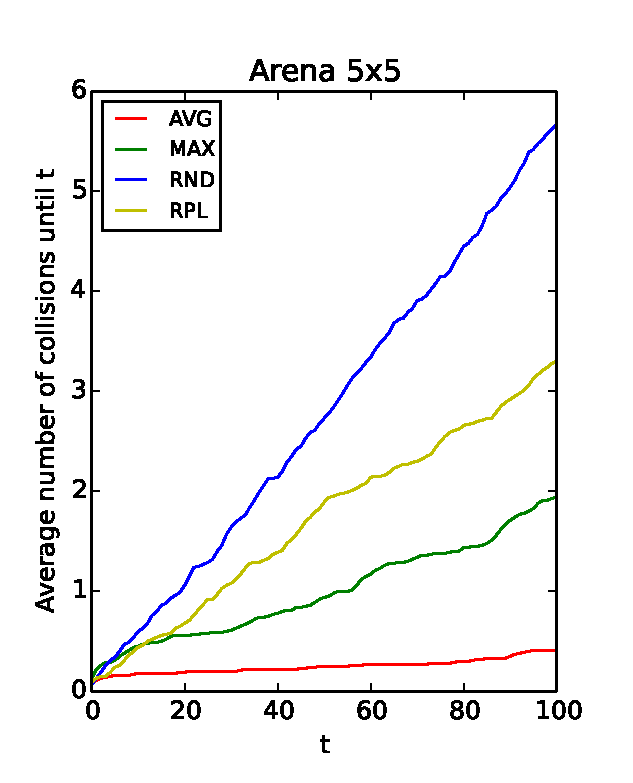
\includegraphics[width=0.42\textwidth]{figures/avoid_C0D5N3.eps}
	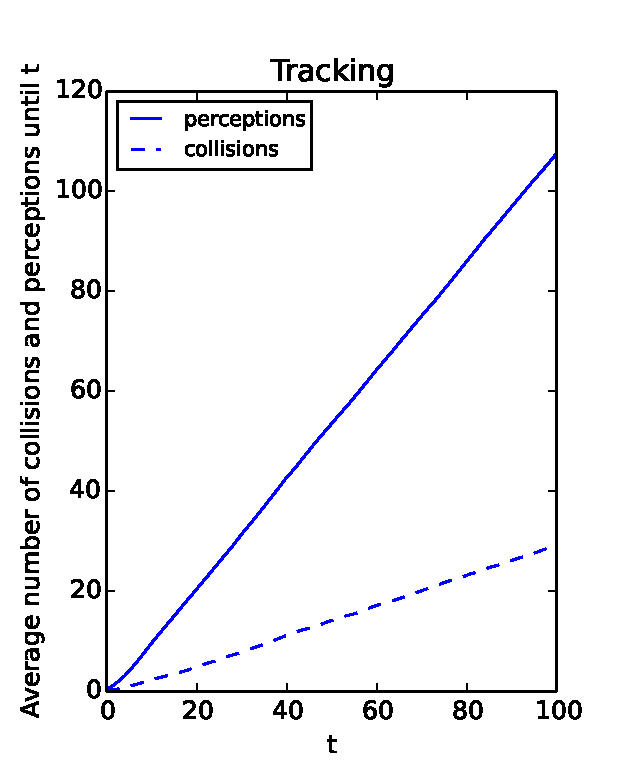
\includegraphics[width=0.42\textwidth]{figures/track_S0N3.eps}
	\caption{Collisions and perceptions with $\varphi_{track}$}
	\label{fig:exp}
\end{figure}

Simulations are written in python, code and data can be downloaded from  \url{http://dropproxy.com/f/BF7}\footnote{The actual code is also in a github repository but we do not report the link for the sake of anonymity.}.% \dots omissis \ldots %~\cite{github}.
%\marginpar{metterlo su dropbox se possibile o trovare un modo di anonimizzare github}
% section case_study (end)

%!TEX root = main.tex
\vspace{-.3cm}
\section{Conclusions and related works} % (fold)
\label{sec:conclusions}

% diamo un framework teorico come metodologia per sistemi adattivi
We have presented a framework for modeling scenarios involving controllable agents, environmental elements and partial perception, where both probabilistic and deterministic behaviours are viable and can be mixed together. Then, we have provided an automatic procedure to build a scheduler for a controllable agent once a \ac{LTL} formula describing the target is given. Since we exploit a model checking algorithm to construct the scheduler, the resulting strategy is guaranteed to maximize the probability to satisfy the target formula.

% offline
The model checking approach allows to split the algorithm into an off-line and an on-line phase, during the former we can evaluate the model and precompute the adaptive scheduler that will be used in the latter to get better performance. Indeed, %the constructed scheduler consists of a light function representation 
the resulting scheduler is just a simple function that maps local states and observations into actions. A possible scenario for using our approach could be to rely on  a high-performance computer to find the appropriate schedulers that could then be sent to small adaptive agents with a low computational power that by themselves would not be able to deal with the model generation phase. Even simpler, the high-performance computer could send the action that has to be executed next directly to the agent, whenever these call for support and communicate their observations.

% target flexibility
Using \ac{LTL} to describe goals gives large expressivity to the framework since conditions on perceptions can be described. Formulae describing avoidance and tracking of moving objects have been introduced and tested, individually and mixed together. Simulations show that multiple objectives can be handled at the same time. 
%
As future work, we would also like to provide a formal language to define composed partially observable models. In this way the designer would be exempted to explicitly write the models, but he would have at the same time the possibility of describing behaviours and observations. Another possible extension of the work is the formula updating in case of a reached (or missed) target.

The model and scheduler generation suffers from a well known scalability issue, and even if this phase does not directly penalize the run-time performance, it could take a prohibitive amount of time. For this reason we plan also to exploit the abstraction technique presented in \cite{KattenbeltKNP10} that permits computing ranges of minimum and maximum probabilities of a given formula and a partition of the states; we want to use an observation-based partition to unburden the workload. 
%Otherwise we could skip the model transformation phase where the state space explosion take place moving the algorithm to the initial configuration of the system where agent and environment are described individually. \marginpar{ultima frase non chiara} 
Otherwise we could aim at analysing the model before the transformation phase (where we can have state space explosion) when agents and environment are described individually.  

\vspace{-.35cm}
\paragraph{Some related work} % (fold)
\label{par:literature_review}
%\emph{Some related work}
Partially observable models like \acp{HMM} \cite{Rabiner90} and \acp{POMDP}~\cite{cassandra1998survey} have been successfully employed in many fields like speech-recognition~\cite{Rabiner90} and activity recognition for ambient assisted living~\cite{vicario2015continuous}.
These models cope with
%the lack of information typical of an adaptive system. 
the adaptive system's typical lack of information.
In particular \acp{POMDP} give the possibility to model the partial knowledge in presence of input and output interactions, as sensing and acting procedures. Finding the optimal scheduler is a problem that has been approached in different ways~\cite{LittmanCK95} since many theoretical limits have been proven to subsist: building the optimal scheduler function is PSPACE-complete in case of finite horizon~\cite{Papadimitriou1987} and determining its existence is undecidable for infinite horizon~\cite{MadaniHC99}.

% model checking on partially observable models
Model checking on \acp{HMM} is proposed in~\cite{ZhangHJ05} together with the extended definitions of branching-time and linear-time logics to include belief states and observation specifications. In this work we adopt a different perspective and we consider observations as label of states. We use classic \ac{LTL} formulae~\cite{Pnueli77} to express properties with probabilistic observations on \acp{POMDP}. 

We did employ model checking techniques to solve a planning problem, 
%this kind of approach has already been proposed in a similar way in~\cite{Bertoli2001,LagoPT02}. In~\cite{Bertoli2001} the model checking techniques are employed to solve a planning problem, 
like in~\cite{Bertoli2001}, but  we further exploit the classical algorithm to solve the same problem at run-time. Also the logic used to formulate agent's objectives differs from the goal language proposed in~\cite{LagoPT02} since we focus on the explicit use of observation signals.

%Linear-time model checking on \acp{POMDP} is just one step toward our aim, that is building a scheduler given an \ac{LTL} formula that describe the objective of the adaptive agent. Indeed, given a formula and the formal model of the system we can reuse the \ac{LTL} model checking algorithm to automatize the computation of a scheduler that can control the adaptive agent.

% paragraph literature_review (end)


% section conclusions (end)

% === BIBLIOGRAPHY ===
\nocite{*}
\bibliographystyle{eptcs}
\bibliography{biblio}
%!TEX root = main.tex
\newpage
\section*{Appendix: Auxiliary notions and proofs}

\subsection*{Preliminary concepts} % (fold)
\label{sub:preliminary_concepts}

\paragraph{Discrete-time Markov chains}
%%%% CILINDRI DTMC
The transition function $T$ induces a measure space on the set of \emph{paths} in a DTMC. 
Given a finite path $\hat\pi = s_0 \dots s_n$, the cylinder set of $\hat\pi = s_0 \dots s_n \in FPaths^{\mathcal{D}}$ is defined as
$$ \mathcal{C}^\mathcal{D}(\hat\pi) = \{ \pi \in Paths^{\mathcal{D}}\ |\ \hat\pi = \pi[..|\hat\pi|-1]\} $$
A $\sigma$-algebra for the possible paths of a Markov chain $\mathcal{D}$ can be defined starting from the cylinder sets.
The probability measure can be finally defined as follows:
\begin{equation}\label{eq:mc_cyl}
Pr^\mathcal{D}_s(\mathcal{C}^\mathcal{D}(s_0\dots s_n)) = 
\begin{cases}
	\prod_{i=1}^n T(s_{i-1})(s_i) \quad \mbox{if } s = s_0 \\
	0 \quad \mbox{otherwise}
\end{cases}
\end{equation}
%%%%
\paragraph{Hidden Markov models}
% arrow notations
%We write $s \rightarrow s'$ when $s$ may go into $s'$, i.e., $T(s)(s') > 0$. We write $s \dashrightarrow o$ when, after a step, state $s$ may generate observation $o$, i.e., $Z(s)(o) > 0$.

% paths set
A path $\pi$ of $\mathcal{H}$ is a sequence $(s_0,o_0),(s_1,o_1)\dots \in (\mathcal{S}\times\mathcal{O})^\omega $ where 
%$s_i \rightarrow s_{i+1}$, $s_i \dashrightarrow o_i$ 
$T(s)(s')>0$, $Z(s)(o)>0$ and $i \in \mathbb{N}$.
Let $Paths^\mathcal{H}$ denote the set of all paths in $\mathcal{H}$. 
%For a path $\pi = (s_0,o_0),(s_1,o_1)\dots \in Paths^\mathcal{H}$, let $\pi_s[i] = s_i$ denote the $(i+1)$st state and $\pi_o[i] = o_i$ denote the $(i+1)$st observation. $FPaths^\mathcal{H} = \{\pi[..n] \ |\ n \in \mathbb{N} \wedge \pi \in Paths^\mathcal{H}\}$ denotes the set of finite paths of $\mathcal{H}$, where $\pi[..n] = (s_0,o_0),(s_1,o_1)\dots(s_n,o_n)$ represents the prefix of $\pi$ of length $n+1$. Let $Paths_\mathcal{O}^\mathcal{H} := \{(\pi_o[0],\pi_o[1]\dots)\ |\ \pi \in Paths^\mathcal{H}\}$ denote the set of observation paths and, defined in an analogous way, $FPaths_\mathcal{O}^\mathcal{H}$ denotes the set of finite observation paths.
%
% cylinder set
and $\hat\pi \in FPaths^\mathcal{H}$ be a finite path on $\mathcal{H}$, we define a \emph{basic cylinder set} on $\hat\pi$ as follows:
$$\mathcal{C}^\mathcal{H}(\hat\pi) = \{ \pi \in Paths^\mathcal{H}\ |\ \forall\ i \in [0..n] . \pi_{i,\mathcal{S}} = \hat\pi_{i,\mathcal{S}} \wedge \pi_{i,\mathcal{O}} = \hat\pi_{i,\mathcal{O}} \} $$

Then we define a probability measure $Pr_s^\mathcal{H} : Cyl^\mathcal{H} \rightarrow [0,1]$ (see \cite{ZhangHJ05}) starting from a state $s \in \mathcal{S}$ as
\begin{equation*}
Pr^\mathcal{H}_s(\mathcal{C}^\mathcal{H}((s_0,o_0)\dots(s_n,o_n))) = \\ 
Pr_s^\mathcal{H}(\mathcal{C}^\mathcal{H}((s_0,o_0)\dots(s_{n-1},o_{n-1})))\ T(s_{n-1})(s_n)\ Z(s_n)(o_n)
\end{equation*}
$$
Pr_s^\mathcal{H}(\mathcal{C}^\mathcal{H}((s_0,o_0))) = \begin{cases}
	Z(s_0)(o_0) \quad \text{if } s_0 = s\\
	0 \quad \text{otherwise}
\end{cases}
$$

By induction on $n$ we obtain:
\begin{equation}\label{eq:prs}
Pr_s^\mathcal{H}(\mathcal{C}^\mathcal{H}((s_0,o_0)\dots(s_n,o_n))) = \begin{cases}
	Z(s_0)(o_0)\prod_{i=1}^{n} T(s_{i-1})(s_i)\ Z(s_i)(o_i) \quad \text{if } s_0 = s \\
	0 \quad \text{otherwise}
\end{cases}
\end{equation}
\begin{proposition}[\cite{ZhangHJ05}]
Let $\mathcal{H}$ be a \ac{HMM} and $Cyl^\mathcal{H}$ be the set of all the basic cylinder sets over $FPaths^\mathcal{H}$, then $(Paths^\mathcal{H},Cyl^\mathcal{H})$ is a measurable space. Moreover, let $Pr^\mathcal{H}_s : Cyl^\mathcal{H} \rightarrow [0,1]$ the probability measure defined in Equation~(\ref{eq:prs}), then $(Paths^\mathcal{H},Cyl^\mathcal{H},Pr_s^\mathcal{H})$ is a probability space.
\end{proposition}

\subsection*{Intermediate results}

The result that follows describe the relation between the probabilistic measure of \acp{POMDP} and \acp{MDP} when the initial state is known.

\begin{proposition}\label{prop:cyl1} 
Let $\mathcal{P}$ be a \ac{POMDP}, $s,s_0,\dots,s_n \in \mathcal{S}_{\mathcal{P}}$, $o_0,\dots,o_n \in \mathcal{O}_{\mathcal{P}}$ and $\eta \in Sched^{\mathcal{P}}$, it holds
	$$ Pr_{s}^{\mathcal{P}_\eta} (\mathcal{C}^{\mathcal{P}_\eta}(s_0,o_0\dots s_n,o_n)) = Z(s_0,o_0) \cdot Pr_{(s,o_0)}^{\widehat{\mathcal{P}}_\eta} (\mathcal{C}^{\widehat{\mathcal{P}}_\eta}((s_0,o_0)\dots(s_n,o_n))) $$
\end{proposition}
%\begin{proposition}\label{prop:cyl2}
%Let $\mathcal{P}$ be a \ac{POMDP}, $s_0,\dots,s_n \in \mathcal{S}_{\mathcal{P}}$, $o_0,\dots,o_n \in \mathcal{O}_{\mathcal{P}}$, $\eta \in Sched^{\mathcal{P}}$
%and let $b \in \Delta(\mathcal{S})$ and $\overline{b} \in \Delta(\mathcal{S}\times\mathcal{O})$ be belief states respectively for $\mathcal{P}_\eta$ and $\widehat{\mathcal{P}}_\eta$ such that $\overline{b}(s,o) = b(s)\cdot Z(s)(o)$, it holds
%	$$ Pr_b^{\mathcal{P}_\eta} (\mathcal{C}^{\mathcal{P}_\eta}(s_0,o_0\dots s_n,o_n)) =  Pr_{\overline{b}}^{\widehat{\mathcal{P}}_\eta} (\mathcal{C}^{\widehat{\mathcal{P}}_\eta}((s_0,o_0)\dots (s_n,o_n)))$$
%\end{proposition}

\begin{proposition}\label{prop:schedset}
Let $\mathcal{P}$ be a \ac{POMDP}, $\widehat{\mathcal{P}}$ be the explicit \ac{MDP} of $\mathcal{P}$ and $\overline{\mathcal{P}}$ be the hidden \ac{MDP} of $\mathcal{P}$, $\widehat{Sched^\mathcal{\overline{P}}} \equiv \{\xi: \mathcal{S}\times\mathcal{O}\rightarrow \mathcal{A}\ |\ \exists\ \eta \in Sched^{\overline{\mathcal{P}}} : \forall\ s \in \mathcal{S},\forall\ o \in \mathcal{O} : \xi(s,o) = \eta(s) \}$, then

$$ \widehat{Sched^\mathcal{\overline{P}}} \subseteq Sched^\mathcal{\widehat{P}} $$
\end{proposition}

% subsection preliminary_concepts (end)
\subsection*{Proofs} % (fold)
\label{sub:proofs}
%Proof of Proposition~\ref{prop:sched}
\begin{proof}[Proposition~\ref{prop:sched}]
The straight implication can be proved as follows
\begin{align*}
	\sum_{m' \in \mathcal{S}_\mathcal{M}} T_{\mathcal{W}}(s,m,\overline\eta(s,\cdot))(s',m')
	= \sum_{m' \in \mathcal{S}_\mathcal{M}} T_{\mathcal{M}}(m,\eta(s))(m') = 1
\end{align*}
The first equivalence is given by definition of $\overline\eta$ and $T_\mathcal{W}$ and we do not lose any component of the sum by hypothesis. In the second step we can exclude the case in which $T_\mathcal{M}(m,\eta(s)) = \bot$ because of the $\mathcal{A}_\mathcal{L}$-responsiveness of $\mathcal{M}$.

The converse implication simply derives from the definition of $T_\mathcal{W}$: since the sum of transition probabilities is one, it exists at least one transition such that
$ T_\mathcal{W}(s,m,\eta(s))(s',m') > 0 $
with positive probability, it follows that $s \xrightarrow{\eta(s)} s'$.
\end{proof}
%Proof of Proposition~\ref{prop:beliefprob}
\begin{proof}[Proposition~\ref{prop:beliefprob}]
	% TODO da risistemare
By hypothesis $b$ has support only on states having $l$ as a state of $\mathcal{L}$, that means that $init(l)$ are all and only the actions that can be executed from $b$. By the definition of $\mathcal{W}$ the transition function $T_\mathcal{W}$ must have probability zero only when states from $\mathcal{L}$ are not connected by an action, then it holds $ \sum_{m \in \mathcal{M}} b(l,m) = 1 \Rightarrow \sum_{m\in \mathcal{M}} b^a(l',m) = 1 $. We conclude the proof since it holds $b^a = 0 \Rightarrow b^{a,o}(s) = 0$ for any action $a$, observation $o$, belief state $b$ and state $s$.
\end{proof}
%Proof of Proposition~\ref{prop:cyl1}
\begin{proof}[Proposition~\ref{prop:cyl1}]
It trivially follows from equations (\ref{eq:mc_cyl}) and (\ref{eq:prs}).
\end{proof}
%Proof of Proposition~\ref{prop:cyl2}
%\begin{proof}
%It trivially follows from definitions (\ref{eq:prb1}) and (\ref{eq:prb2}).	
%\end{proof}
%Proof of Theorem~\ref{teo:pmins}

\begin{proof}[Proposition~\ref{prop:schedset}]
	We define $\widehat{Sched^{\overline{\mathcal{P}}}}$ as a set of schedulers for explicit \acp{MDP} that chose actions only relying on the current state mimicking the behavior of schedulers for the hidden \ac{MDP} of $\overline{\mathcal{P}}$. This kind of construction considers only schedulers for the explicit \ac{MDP} that choose the same action from the same state ignoring the observation. 
	We can split schedulers in $Sched^{\mathcal{\widehat{P}}}$ in two partitions, schedulers that always take the same decisions in the same state and schedulers that take at least a different decision from the same state with different observations. We generate the former category excluding the latter, it follows that $\widehat{Sched^{\overline{\mathcal{P}}}} \subseteq Sched^{\widehat{\mathcal{P}}}$
\end{proof}

\begin{proof}[Theorem~\ref{teo:pmins}]

%	$$ 
%	\begin{array}{lll}
%		p_{min}^\mathcal{M}(s, \varphi) &=& \inf_\eta Pr_s^{\mathcal{M}_\eta}\{\pi \in Paths^\mathcal{M}\ |\ \pi \models \varphi\} \\
%		&=& \min_\eta Pr_s^{\mathcal{M}_\eta}\{\pi \in Paths^\mathcal{M}\ |\ \pi \models \varphi\} 
%	\end{array}
%	$$

We rely on Proposition~\ref{prop:cyl1} for this proof, since it shows that cylinders probabilities in \acp{DTMC} and \acp{HMM} differ only of a multiplicative factor.

During the passages the notation $psat(\varphi) \in (\mathcal{S}_{\mathcal{P}}\times\mathcal{O}_\mathcal{P})^*$ is used to define the set of finite paths of maximal length that satisfy $\varphi$.

$$
\begin{array}{lll}
	p^{\widehat{\mathcal{P}}}_{min}((s,o),\varphi) &=& \displaystyle \inf_{\xi \in Sched^{\widehat{\mathcal{P}}}} Pr_{(s,o)}^{\widehat{\mathcal{P}}_{\xi}}\{\pi \in Paths^{\widehat{\mathcal{P}}}\ |\ \pi \models \varphi\} \\
	%&& \{\text{We apply \cite[Lemma 10.102]{Katoen-Baier} to $\widehat{\mathcal{P}}$ that is a \ac{MDP}} \\
	%&& \text{by Definition~\ref{def:emdp}}\} \\
	%&=& \displaystyle \inf_{\xi \in Sched^{\widehat{\mathcal{P}}}} Pr_{(s,o)}^{\widehat{\mathcal{P}}_{\xi}}\{\pi \in Paths^{\widehat{\mathcal{P}}}\ |\ \pi \models \varphi\} \\
	&& \{ \text{We reformulate the set of paths as the union of} \\
	&& \text{cylinder sets obtained by } \varphi \} \\
	&=& \displaystyle \inf_{\xi \in Sched^{\widehat{\mathcal{P}}}} \sum_{\hat\pi \in psat(\varphi)} Pr_{(s,o)}^{\widehat{\mathcal{P}}_{\xi}}(\mathcal{C}^{\widehat{\mathcal{P}}_{\xi}}(\hat\pi)) \\
	&& \{\text{By the definition of probability measure} \\
	&& \text{on Markov chains (\ref{eq:mc_cyl})}\} \\
	&=& \displaystyle \inf_{\xi \in Sched^{\widehat{\mathcal{P}}}} \sum_{\substack{\hat\pi \in psat(\varphi) \wedge \\ \hat\pi = s,o,s_1,o_1\dots s_n,o_n }} \prod_{i=1}^n \widehat{T}((s_{i-1},o_{i-1}),\xi(s_{i-1},o_{i-1}))(s_i,o_i) \\
	&& \{\text{By Definition~\ref{def:emdp} of $\widehat{T}$ and Proposition~\ref{prop:schedset}}\} \\
	&\geq& \displaystyle \inf_{\eta \in \widehat{Sched^{\mathcal{\overline{P}}}}} \sum_{\substack{\hat\pi \in psat(\varphi) \wedge \\ \hat\pi = s,o,s_1,o_1\dots s_n,o_n}} \prod_{i=1}^n T(s_{i-1},\eta(s_{i-1}))(s_i) Z(s_i)(o_i) \\
\end{array}
$$

In the following chain of equations we use the previous result to connect the minimum probability on $\mathcal{P}$ with a weighted sum of minimum probabilities on $\widehat{\mathcal{P}}$. %To do that we need to specify that, for any action $a$ $T(s,a)$

$$
\begin{array}{lll}
	p^{\mathcal{P}}_{min}(s,\varphi) &=& \displaystyle \inf_{\eta \in Sched^{\mathcal{\overline{P}}}} Pr_s^{\mathcal{P}_{\eta}}\{\pi \in Paths^{\mathcal{P}}\ |\ \pi \models \varphi\} \\
	&& \{ \text{We reformulate the set of paths as the union} \\ 
	&& \text{of cylinder sets obtained by $\varphi$} \} \\
	&=& \displaystyle \inf_{\eta \in Sched^{\mathcal{\overline{P}}}} \sum_{\hat\pi \in psat(\varphi)} Pr_s^{\mathcal{P}_\eta}(\mathcal{C}^{\mathcal{P}_\eta}(\hat\pi)) \\
	&& \{ \text{By the definition of probability measure on \ac{HMM} (\ref{eq:prs})} \} \\
	&=& \displaystyle \inf_{\eta \in Sched^{\mathcal{\overline{P}}}} \sum_{\substack{\hat\pi \in psat(\varphi) \wedge \\ \hat\pi = s,o_0,s_1,o_1\dots s_n,o_n}} Z(s)(o_0) \prod_{i=1}^n T(s_{i-1},\eta(s_{i-1}))(s_i) Z(s_i)(o_i) \\
	&=& \displaystyle \inf_{\eta \in Sched^{\mathcal{\overline{P}}}} \sum_{\tilde{o}\in\mathcal{O}} \sum_{\substack{\hat\pi \in psat(\varphi) \wedge \\ \hat\pi = s,\tilde{o},s_1,o_1\dots s_n,o_n}} Z(s)(\tilde{o}) \prod_{i=1}^n T(s_{i-1},\eta(s_{i-1}))(s_i) Z(s_i)(o_i) \\
	&& \{\text{Since the initial state $s$ does not change we can swap} \\ 
	&& \text{the sum with the infimum operator}\} \\
	&=& \displaystyle \sum_{\tilde{o}\in\mathcal{O}} Z(s)(\tilde{o}) \inf_{\eta \in Sched^{\mathcal{\overline{P}}}}  \sum_{\substack{\hat\pi \in psat(\varphi) \wedge \\ \hat\pi = s,\tilde{o},s_1,o_1\dots s_n,o_n}} \prod_{i=1}^n T(s_{i-1},\eta(s_{i-1}))(s_i) Z(s_i)(o_i) \\
	&& \{\text{By the result of the previous equation}\} \\

	&\leq& \displaystyle \sum_{\tilde{o}\in\mathcal{O}} Z(s)(\tilde{o}) \cdot p_{min}^{\widehat{\mathcal{P}}}((s,\tilde{o}),\varphi) \\
\end{array}
$$
\end{proof}
%Proof of Corollary~\ref{cor:infmin}
\begin{proof}[Corollary~\ref{cor:infmin}]
From \cite[Lemma 10.102]{Katoen-Baier} we know that, for a \ac{MDP} $\mathcal{M}$, it always exists a finite-memory scheduler that minimize the probabilities for $\varphi$. The result directly follows from it and Theorem~\ref{teo:pmins}.
\end{proof}
% subsection proofs (end)

\end{document}
